%%%%%%%%%%%%%%%%%%%%%%%%%%%%%%%%%%%%%%%%%%%%%%%%%%%%%%%%%%%%%%%%%%%%%%
% COMP 3804
% February 13, 2012
% Final Exam Notes
% By Alexis Beingessner
%    Simon Pratt
%%%%%%%%%%%%%%%%%%%%%%%%%%%%%%%%%%%%%%%%%%%%%%%%%%%%%%%%%%%%%%%%%%%%%%
\documentclass[11pt]{book}

\usepackage{geometry}
\geometry{verbose,tmargin=1in,bmargin=1in,lmargin=.5in,rmargin=.5in}
\usepackage[pdftex]{graphicx}
\usepackage{fancyhdr}
\usepackage{fix-cm}
\usepackage{amsmath}
\usepackage{enumerate}
\usepackage{amsthm}
\usepackage{amssymb}
\usepackage{parskip}
%\usepackage{algorithm}
\usepackage{algorithmic}
\usepackage{multicol}
%\usepackage{newclude} % \include without \clearpage
%\usepackage{ulsy} % needed for \blitza

%%%%%%%%%%%%%%%%%%%%%%%%%%%%%%%%%%%%%%%%%%%%%%%%%%%%%%%%%%%%%%%%%%%%%%
% Question and Answer environments
%%%%%%%%%%%%%%%%%%%%%%%%%%%%%%%%%%%%%%%%%%%%%%%%%%%%%%%%%%%%%%%%%%%%%%

\newcounter{ques}
\newenvironment{question}{\stepcounter{ques}{\bf Question \arabic{ques}:}\vspace{1mm}\fontsize{8}{8}\selectfont}{}
\newenvironment{subquestion}{\fontsize{8}{8}\selectfont}{}
\newenvironment{answer}{{\bf Answer:}\fontsize{12}{12}\selectfont}{}

%%%%%%%%%%%%%%%%%%%%%%%%%%%%%%%%%%%%%%%%%%%%%%%%%%%%%%%%%%%%%%%%%%%%%%
% Theorem, Lemma and Definitions
%%%%%%%%%%%%%%%%%%%%%%%%%%%%%%%%%%%%%%%%%%%%%%%%%%%%%%%%%%%%%%%%%%%%%%

\newtheorem{theorem}{Theorem}[chapter]
\newtheorem{lemma}{Lemma}[chapter]
\theoremstyle{definition}
\newtheorem{definition}{Definition}[chapter]
\newtheorem{claim}{Claim}[chapter]

%%%%%%%%%%%%%%%%%%%%%%%%%%%%%%%%%%%%%%%%%%%%%%%%%%%%%%%%%%%%%%%%%%%%%%
% Fix for amsthm and parskip
% URL: http://tex.stackexchange.com/questions/22119/how-can-i-change-the-spacing-before-theorems-with-amsthm
%%%%%%%%%%%%%%%%%%%%%%%%%%%%%%%%%%%%%%%%%%%%%%%%%%%%%%%%%%%%%%%%%%%%%%

\makeatletter
\def\thm@space@setup{%
  \thm@preskip=\parskip \thm@postskip=0pt
}
\makeatother

%%%%%%%%%%%%%%%%%%%%%%%%%%%%%%%%%%%%%%%%%%%%%%%%%%%%%%%%%%%%%%%%%%%%%%
% Header/footer
% Mostly taken from: 
%  https://texblog.wordpress.com/2007/11/07/headerfooter-in-latex-with-fancyhdr/
%%%%%%%%%%%%%%%%%%%%%%%%%%%%%%%%%%%%%%%%%%%%%%%%%%%%%%%%%%%%%%%%%%%%%%
\pagestyle{fancyplain}
\setlength{\headheight}{14pt}
\fancyhead{}             % clear header
\fancyfoot{}

\fancyhead[L]{COMP3804}
\fancyhead[C]{Page \thepage }
\fancyhead[R]{Alexis Beingessner \\ Simon Pratt}

%%%%%%%%%%%%%%%%%%%%%%%%%%%%%%%%%%%%%%%%%%%%%%%%%%%%%%%%%%%%%%%%%%%%%%
% Pretty math macros
%%%%%%%%%%%%%%%%%%%%%%%%%%%%%%%%%%%%%%%%%%%%%%%%%%%%%%%%%%%%%%%%%%%%%%
\newcommand{\summ}[2]{\ensuremath{\displaystyle\sum\limits_{#1}^{#2}}} 
%pretty summation

%%%%%%%%%%%%%%%%%%%%%%%%%%%%%%%%%%%%%%%%%%%%%%%%%%%%%%%%%%%%%%%%%%%%%%
% Document
%%%%%%%%%%%%%%%%%%%%%%%%%%%%%%%%%%%%%%%%%%%%%%%%%%%%%%%%%%%%%%%%%%%%%%

\title{Algorithms Notes}
\date{}
\author{Alexis Beingessner\\Simon Pratt}

\begin{document}
\maketitle
\tableofcontents
\begin{multicols}{2}
  
  \chapter{Two Fibonaccis}

$fib(n):$
\begin{algorithmic}
\IF { $ n=0 $ or $ n=1 $ }
\RETURN $n$
\ELSE
\RETURN $fib(n-1) + fib(n-2)$
\ENDIF
\end{algorithmic}

We can state a recurrence for this algorithm:

\begin{align*}
T(n) 
&= T(n-1) + T(n-2) + O(1) \\
&\geq fib(n-1) + fib(n-2) \\
&= fib(n)
\end{align*}

$fib2(n):$
\begin{algorithmic}
\IF { $ n = 0 $ }
\RETURN 0
\ENDIF
\STATE create array $f[0 .. n]$
\STATE $f[0] \leftarrow 0, f[1] \leftarrow 1$
\FOR { $ i \leftarrow 2$ to $n$ }
\STATE $f[i] \leftarrow f[i-1] + f[i-2]$
\ENDFOR
\RETURN $f[n]$
\end{algorithmic}

Addition of two numbers in the preceding algorithm takes constant time
until the values exceed the maximum value that can be stored in a
word.  After which, we need to consider how values of arbitrary length
are added.
                   % done
  \chapter{Integer Multiplication}

Let us consider an integer $X$ which is composed of $X_L$ which are
the leftmost bits of $X$, and $X_R$ which are the rightmost bits of
$X$.

\begin{displaymath}
X = X_L | X_R
\end{displaymath}

We can multiply integers $X,Y$ as follows:

\begin{align*}
XY
&= (2^{n/2}X_L + X_R)(2^{n/2}Y_L + Y_R) \\
&= 2^n X_LY_L + 2^{n/2}X_LY_R + 2^{n/2}X_RY_L + X_RY_R \\
&= 2^n X_LY_L + 2^{n/2}(X_LY_R + X_RY_L) + X_RY_R \\
\end{align*}

Which gives the recurrence

\begin{align*}
T(n)
&= 4T(n/2) + O(n) \\
&\leq 4T(n/2) + cn \\
&\leq 4(4T(n/4) + cn/2) + cn \\
&\leq 4(4(4T(n/8) + cn/4) + cn/2) + cn \\
&\leq 64T(n/8) + cn(1 + 2 + 4) \\
&... \\
&\leq 4^iT(n/2^i) + cn(1 + 2 + ... + 2^{i-1})
\end{align*}

Where $i$ is the number of times we can divide $n$ by 2, or $log_2n$.

\begin{align*}
T(n)
&\leq 4^{log_2n}T(n/2^{log_2n}) + cn(1 + 2 + ... + 2^{log_2n-1}) \\
&\leq n^{log_24}T(n/n^{log_22}) + cn \summ{i=0}{log_2n-1} 2^i \\
&\leq n^2T(1) + cn 2^{log_2n} \\
&\leq n^2T(1) + cn n^{log_22} \\
&\leq n^2T(1) + cn^2 \\
&\leq n^2(T(1) + c) \\
&\leq n^2(O(1) + c) \\
&\leq O(n^2)
\end{align*}

Can we do better?  Yes.

We need: $X_LY_L, X_RY_R,$ and $X_LY_R + X_RY_L$

Observe: 
%
\begin{align*}
&(X_L + X_R)(Y_L + Y_R) - X_LY_L - X_RY_R \\
&= X_LY_L + X_RY_L + X_LY_R + X_RY_R - X_LY_L - X_RY_R \\
&= X_RY_L + X_LY_R
\end{align*}

Since we must compute $X_LY_L$ and $X_RY_R$ anyway, this saves us an
entire multiplication.  Reducing our recurrence from $T(n) = 4T(n/2) +
O(n)$ to $T(n) = 3T(n/2) + O(n)$.

We can solve this new recurrence as follows:

\begin{align*}
T(n)
&= 3T(n/2) + O(n) \\
&\leq 3T(n/2) + cn \\
&\leq 3(3T(n/4) + cn/2) + cn \\
&\leq 3^iT(n/2^i) + cn(1 + 3/2 + ... + (3/2)^{i-1}) \\
&\leq 3^{log_2n}T(n/2^{log_2n}) + cn(1 + 2 + ... + (3/2)^{log_2n-1}) \\
&\leq n^{log_23}T(1) + cn \summ{i=0}{log_2n-1} (3/2)^i \\
&\leq n^{log_23}T(1) + cn (3/2)^{log_2n} \\
&\leq n^{log_23}T(1) + cn n^{log_2(3/2)} \\
&\leq n^{log_23}T(1) + cn n^{log_23 - log_22} \\
&\leq n^{log_23}T(1) + cn n^{log_23 - 1} \\
&\leq n^{log_23}T(1) + cn n^{log_23}n^{-1} \\
&\leq n^{log_23}(T(1) + cn/n) \\
&\leq n^{log_23}(T(1) + c) \\
&\leq O(n^{log_23})
\end{align*}
      % done
  \chapter{Solving Recurrences}

\section{The Master Theorem}

If $T(n) = aT(\frac{n}{b}) + O(n^d)$, then

\begin{math}
T(n) = \left\{
\begin{array}{l l}
O(n^d)       & \quad \text{if} d > log_ba \\
O(n^d logn)  & \quad \text{if} d = log_ba \\
O(n^{log_ba}) & \quad \text{if} d < log_ba \\
\end{array} \right.
\end{math}

\section{Recursion Tree}

We can reason about a recurrence of the form: $ T(n) = aT(\frac{n}{b})
+ f(n) $ where $ a \geq 0, b > 0 $ with the following recursion tree:

{
  % Current graphic is hand-drawn by John Howat.
  % Should replace asap with a nicer diagram
  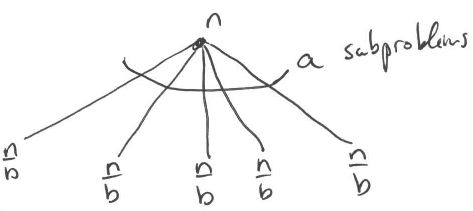
\includegraphics[scale=1.2]{recursion_tree}
  %\caption{A recursion tree representing a recursions on n/b elements}
  \label{fig:recursion_tree}
}

This tree has the following properties:

\begin{enumerate}
\item The number of nodes at level $i$: $a^i$
\item Work done at each node of level $i$: $f(\frac{n}{b^i})$
\item Number of levels: $log_bn$
\item Number of leaves: $n^{log_ba}$
\end{enumerate}

We can use this information to solve the recurrence:

\begin{align*}
T(n)
&= \summ{i=0}{log_bn} 
(\text{\# nodes at level } i) 
(\text{work done at level } i) \\
&= \summ{i=0}{log_bn} a^i f(\frac{n}{b^i})
\end{align*}
                 % done
  \chapter{Heaps}

For the purposes of generality, instead of referring to 
elements that are ``greater than" or ``less than" others,
we will simply say that they are ``better than" or ``worse than"
others. For any particular ordering, the ``best" element is desired first.
A Heap is a binary tree that satisfies the following properties:

\begin{itemize}
\item The root of a heap is better than its two children (the heap property)
\item The children of the root are also heaps  
\item A heap is a complete binary tree (only the last level may not be full, 
and all elements in the last level are on the left)
\end{itemize}

A heap differs from most binary trees in that it provides no particular
ordering of the elements, but rather guarantees that the best element is
at the root. Further, while heaps are usually discussed and defined
as binary trees, they need not be implemented as such.
A heap can in fact be implemented as an array with no performance reduction.
Contrary to standard theoretical convention, we will be using 0-indexed arrays
rather than 1-indexed arrays. That is to say, the indexing will reflect how
most programming languages perform indexing (0 is the first element, not 1).
To represent a heap as an array, we can implement a simple indexing. 
If an element is at the $i$th
index in the array, its left and right child are at the $2i+1$th and $2i+2$th 
indexes respectively. By placing the root at the $0$th index, all others follow.
This is depicted below.
{
  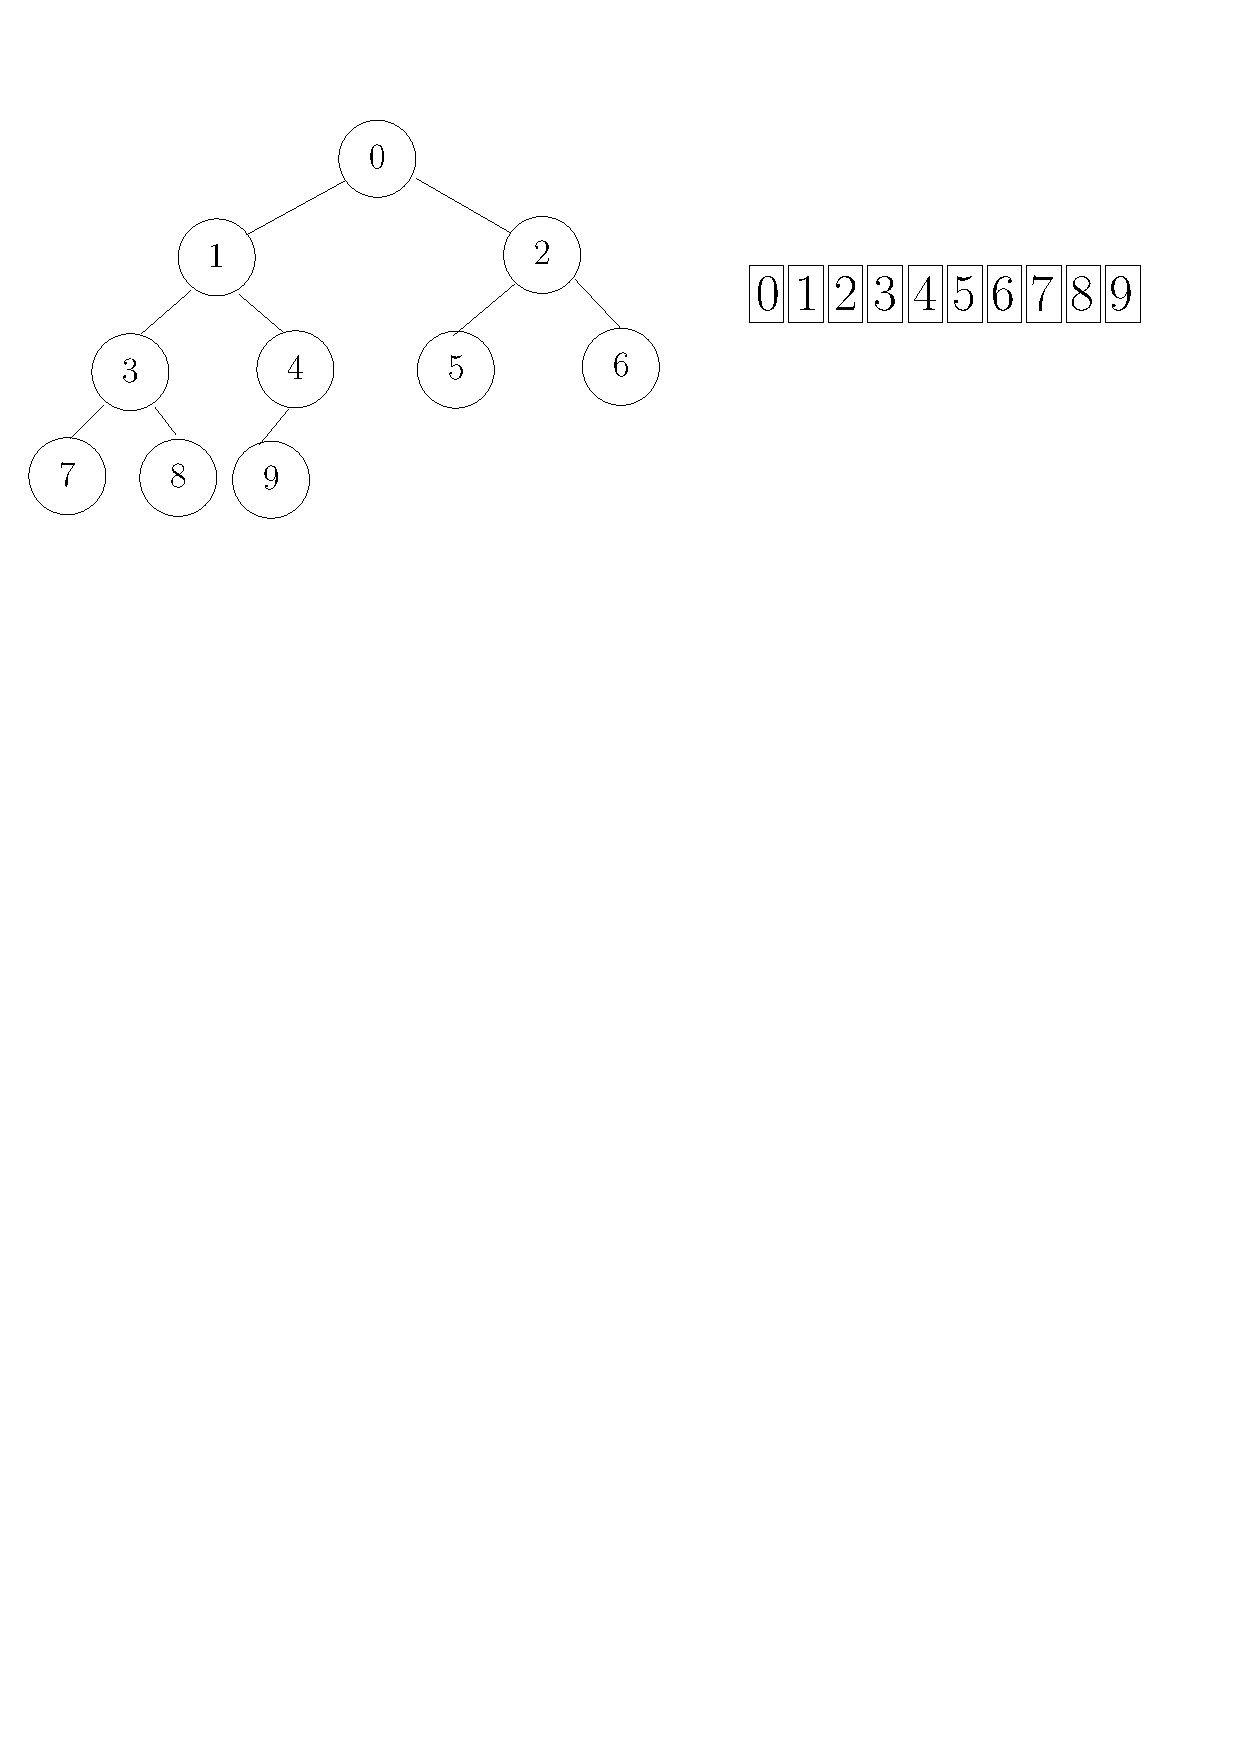
\includegraphics[scale=0.5]{heapTreeArray}
  %\caption{The mapping of a binary tree to an array}
  \label{fig:heapTreeArray}
}
Heaps are commonly used to implement priority queues, because they do the
minimum amount of work required to keep track of the best element.

\section{How to Implement a Heap}

A heap must support the following operations

\begin{itemize}
\item $best()$: returns the best element in the heap
\item $pop-best()$: removes the best element in the heap
\item $insert(x)$: inserts $x$ into the heap
\end{itemize}

From the definition of a heap, we know the we can easily implement
$best()$ by returning the root of the heap, which should take $O(1)$
time.  However the other operations are less obvious.

To $insert(x)$ recall that a heap must be complete, therefore, if a
new element is added, it must be added to the left-most available
space in the last row of the heap. However, the heap property may now
be violated.  If the new element $x$ is worse than its parent $y$, the
heap property is satisfied and we may stop. However if it is not
satisfied we may swap $x$ with $y$ and recurse on $x$'s new
position. This works because we know that $y$ is better than all of
$x$'s children, because the heap property was satisfied before $x$ was
added. Further, because $x$ is better than $y$, it is also better than
all of $y$'s children. However $x$ may still be better than its new
parent, so we must recurse. If $x$ is the new best element, it will
eventually reach the root. Because heaps are complete, this operation
will take $O(\log n)$ time, as this is the height of the heap.

To $pop-best()$, we may simply remove the root, however this
completely destroys the entire heap. Instead, we will swap the root
with the bottom-left-most element, $y$. Now removing the best element
leaves us with a still complete tree. However the heap property has
likely been violated once more. If $y$ is better than both its
children, then we may stop. However, if not, we shall swap $y$ with
its best child and recurse on $y's$ new position. Because the element
we swap with $y$ is better than both $y$ and the other child, the heap
property has been satisfied for this sub-heap. However, the heap
property may still be violated for $y's$ new sub-heap, so we must do
this again, until $y$ is the root of a valid heap. Once more, this
operation requires $O(\log n)$ time, as it must at worse traverse the
entire height of the tree.

Therefore, a heap may support $best()$ in $O(1)$ time, $insert(x)$ 
in $O(\log n)$ time, and $pop-best()$ in $O(\log n)$ time.

\section{Building a Heap}

Now that we can support all the operations that a heap must implement,
it would be nice to be able to actually construct one given a list of $n$
elements. A na\"ive approach is to simply call $insert(x)$ on every element
in the list. However, since $insert(x)$ requires $O(\log n)$ time, this will
require $O(n \log n)$ time. These seems pretty bad, considering one can find
the best element in a list by brute force in $O(n)$ time. Can we achieve a
construction time comparable to the brute force time?
Instead of building the heap top down with $insert$, we can build it from the
bottom up. Remark that a single element is a valid heap. If we were to try to
build from the bottom up, we could first take the last $n/2$ elements in the
list. All of these elements are their own valid and complete heaps,
and we therefore do not need to do anything to them.
To add the next $n/4$ elements, we simply perform
the procedure we did in $pop-best$ to fix the fact that the new root might
be violating the heap property, knowing that all the elements below it are
valid heaps. By repeating this process until we reach the first element in
the list, we will have created a valid heap on $n$ elements.

Because we are doing very little work for the majority of the elements, we end
up doing only $O(n)$ work over all, which is optimal, as this is the amount of
time required to find the best element.

\section{Heapsort}

Another nice property of a heap is that once one has been implemented,
it provides a very simple procedure for sort elements.
A simple algorithm to do this to construct a heap on the list and then simply
return $best$ and then call $pop-best$ over and over until there are no more
elements in the heap.
In fact, since our algorithm for building the heap is in-place and takes $O(n)$
time, and our remove method leaves the best element at the end of the array,
by simply building a heap on the input array and calling $pop-best$ $n$ times,
we will be left with a reverse sorted array in $O(n \log n)$ time. 
This algorithm is particularly excellent because it requires no extra space,
runs deterministically, and is worst-case optimal.

                       % done
  \chapter{Selection}

Consider the following problem: given an array $A$ of $n$ elements,
output the $i$-th smallest element of $A$.

As a simple first solution, we can sort $A$ and then return $A[i]$.
Since sorting takes $O(nlogn)$ time and returning $A[i]$ takes $O(1)$
time, this solution takes $O(nlogn) + O(1) = O(nlogn)$ time.

But it should be easy to see that we can do better in specific cases
like $i=1$ or $i=n$.  Simply iterate once over the array and store the
minimum ($i=1$) or maximum ($i=n$) value.  Since looking at a
particular element of the array takes $O(1)$ time, and we look at all
$n$ elements, this takes total $n \cdot O(1) = O(n)$ time.

We can also tell that this is optimal, because we know that to
determine the $i$-th element, we need to look at all $n$ elements in
the array, so we have a lower bound of $\Omega (n)$ time.

But is this possible in general, for any value of $i$?  Yes.

Suppose in linear time we can find element $x$ such that

{
  % Current graphic is hand-drawn by John Howat.
  % Should replace asap with a nicer diagram
  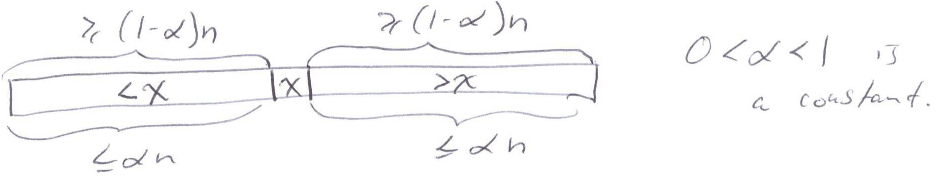
\includegraphics[scale=0.6]{selection}
  %\caption{Desirable properties of element x.}
  \label{fig:selection}
}

$x$ is somewhere around the middle of the array, and is preceded only
by elements smaller than $x$, and followed only by elements larger
than $x$.  We also know that there are $ \geq (1-\alpha)n $ and $ \leq
\alpha n $ elements both before and after $x$.

We can calculate this $x$ as follows:

\begin{enumerate}

\item Split $A$ into groups of 5.  There will be $\frac{n}{5}$ of
  these groups.
\item Compute the median $m_j$ of each group $M_j$ for $ 1 \leq j \leq
  \frac{n}{5} $.
\item Compute the median $x$ of $m_1,m_2,...,m_{n/5}$.

\end{enumerate}

It should be clear that step 1 takes constant time, step 2 takes
constant time for each group of constant size and $O(n)$ time total
for all $\frac{n}{5}$ groups, and step 3 takes $T(n/5)$ time.

\begin{claim}
This $x$ has the properties we needed above.
\end{claim}

\begin{proof}

We know that $\frac{1}{2}$ of $m_j$ are smaller than $x$, and since
there are $ \frac{n}{5} m_j$s, we know $\frac{n}{10}$ of $m_j$ are $
\leq x $.

So for each $m_j$ where $m_j \leq x$ 

\begin{itemize} 

\item there are 3 elements that are $ \leq m_j $
\item so 3 (or more) elements are $ \leq x $

\end{itemize}
%
\end{proof}
%
Now we must put $x$ into its position in the array using partitioning.
As a side note, partitioning is used in quicksort.

\begin{enumerate}

\item Find $x$, put it at the end
\item Partition elements around $x$
\item Put $x$ into its proper position

\end{enumerate}

We now have an $x$ that satisfies the properties we needed, and it is
properly located at position $q$ in $A$.  We are left with 3 cases:

\begin{enumerate}

\item If $i = q$: $x$ is the $i$-th element of $A$.
\item If $i < q$: recurse on the subarray which is $ < x $

\item If $i > q$: recurse on the subarray which is $ > x $, and $ i
  \leftarrow i - q $

\end{enumerate}

This last step gives a recurrence of $ T \left( \frac{7n}{10} \right)
$ in the worst case because at least $ \frac{3n}{10} $ elements in $A$
are smaller than $x$.

\section{Analysis}

We now have the following recurrence:
%
\begin{displaymath}
T(n) = T \left( \frac{n}{5} \right) +T \left( \frac{7n}{10} \right) + O(n)
\end{displaymath}

\begin{claim}
$ T(n) \leq cn $
\end{claim}

\begin{proof}
\begin{align*}
T(n)
&= dn + T \left( \frac{n}{5} \right) +T \left( \frac{7n}{10} \right) \\
&\leq dn + c \frac{n}{5} + c \frac{7n}{10} \\
&= dn + \frac{9}{10}cn \\
&= cn \left( \frac{d}{c} + \frac{9}{10} \right)
&\leq cn
\end{align*}

As long as

\begin{align*}
\frac{d}{c} + \frac{9}{10} &\leq 1 \\
\frac{d}{c} &\leq \frac{1}{10} \\
10 d &\leq c
\end{align*}
\end{proof}

\section{What is special about 5?}

First of all, we need an odd number for there to be a median.
Secondly, notice:
%
\begin{displaymath}
\frac{1}{5} + \frac{7}{10} = \frac{9}{10} < 1
\end{displaymath}

Dividing into groups of 3 doesn't work because:
%
\begin{displaymath}
T(n) = O(n) + T(n/3) + T(2n/3) = \Theta(nlogn)
\end{displaymath}

Dividing into groups of 7 actually does work because:
%
\begin{displaymath}
T(n) = O(n) + T(n/7) + T(5n/7) = \Theta(n)
\end{displaymath}
                   % done
  \chapter{Union-Find}

Consider the following problem. Given $n$ disjoint sets of 1 element each,
perform $n$ unions and then $m$ queries for what set a given element is in.
We will call these two operations $union(A,B)$ and $find(x)$. 

\section{Approach 1: Linked Lists}
Our first
approach to this problem is to describe our sets as linked lists. We know
we can combine linked lists quite quickly, so this seems ideal for $union$. 
All we must do is have the head of $B$ point to the tail of $A$, which can be
done in constant time.
However, linked lists are not particularly well suited for $find$. To resolve
this, at every node we shall store a $back pointer$ to the linked list 
the node is part of. This allows us to perform $find$ in constant time. 
However, now $union$ needs some extra work.
When we call $union(A,B)$, we will now walk through $B$ and fix all of its
back pointers to point to $A$. This will take time linear in the size of $B$.

Given $n$ sets, what is the worst possible way to $union$ them? Well, since
the run time $union$ is linear in the size of the second list, adversarial
we can
do is to $union$ every individual element with the current unioned set. For
instance, $union(D,union(C,union(A,B)))...$. Clearly this will require
$O(\summ{i=1}{n-1}i)$, which is $O(n^2)$. If we then perform $m$ $find$s, all
of which take $O(1)$ time, we will have performed $n$ $union$s and $m$ $find$s
in $O(n^2 + m)$ time.

\section{Approach 2: Better Linked Lists}
Somehow our first approach was na\"ive, which allowed us to ``game" the system
to create a very bad result for the $union$s. To get a better result, we will
make a slight modification to our $union$ algorithm. Instead of blindly
attaching $B$ to the end of $A$, we will attach the smaller set to the larger.
This fixes our adversarial approach, but is it actually better? 

Consider how frequently we need to change the back pointers on an individual
node. At first, it is part of a set of size one, and will have to change its
pointer when unioned to a set of size $\geq 1$, placing it in a set
of size $\geq 2$. The next time it will be changed is when it is unioned
to a set of size $\geq 2$, then $\geq 4$ and so on. The last time will be
when it is unioned to a set of size $\geq n/2$ after which we can not find
another set of large enough size to change it again. Therefore each
back pointer needs to be changed $O(\log n)$ times at worst. Since there
are $n$ back pointers, this new approach only require $O(n \log n)$
time to perform the unions. Since the $find$ operation is not effected,
our approach now performs $n$ $union$s and $m$ $find$s
in $O(n \log n + m)$ time.

\section{Approach 3: Trees}
Having to fix back pointers is still fairly wasteful, what if we didn't have
to? Instead of implementing our sets as linked lists, we can instead
use trees. Each set will be a node with either the name of the set, or a
pointer to its parent. When we perform $union(A,B)$, we will simply
replace the name of the shorter set with a pointer to the head of the taller
set. Since we are just changing a pointer, this will only take $O(1)$ time.
Our $find$ algorithm, however, will now have to walk from the node all the way
to the root of the tree it is in to find out what list it is in. By a
similar argument from the previous section, the height of our tree will only
ever be $\log n$. 
Therefore this approach can support $n$ $union$s and $m$ $find$s
in $O(n + m \log n)$ time.

\section{Approach 4: Path Compression}
Our $union$ algorithm is optimal using the tree approach, but it has
made our $find$ algorithm suffer. To fix this, we make a simple observation.
Since our find algorithm must already walk through several nodes in the tree,
once we get to the root we can, without worsening the time,
relabel all of their pointers to point directly to the root. This approach
is called $path compression$. This will make
subsequent queries on these elements and their children substantially faster.
The analysis of this algorithm is beyond the scope of this class, but
evidently it  can support $n$ $union$s and $m$ $find$s
in $O(n + m \alpha(n))$ time. Where $\alpha$ is the inverse Ackermann function. 
Although $\alpha(n)$ tends towards infinity as $n$ does, for any ``practical"
$n$ it is at most $4$. It turns out that this is in fact optimal for the
union-find problem.
                  % done
  \chapter{Graphs}

A \emph{graph} is an ordered pair $G=(V,E)$ where $V$ is a set of
\emph{vertices} and $E$ is a set of \emph{edges}.  An edge is a pair
of vertices which are said to be \emph{adjacent}.  An edge is said to
be \emph{incident} on its component vertices.  Usually we consider
edges to be unordered, in which case the graph is undirected and an
edge $\{A,B\}$ connects $A$ to $B$ and $B$ to $A$.  For example:

\begin{align*} 
V &= \{ A, B, C \} \\ E &= \{ (A, B), (B, C) \} 
\end{align*}

Which can be represented more visually:

{
  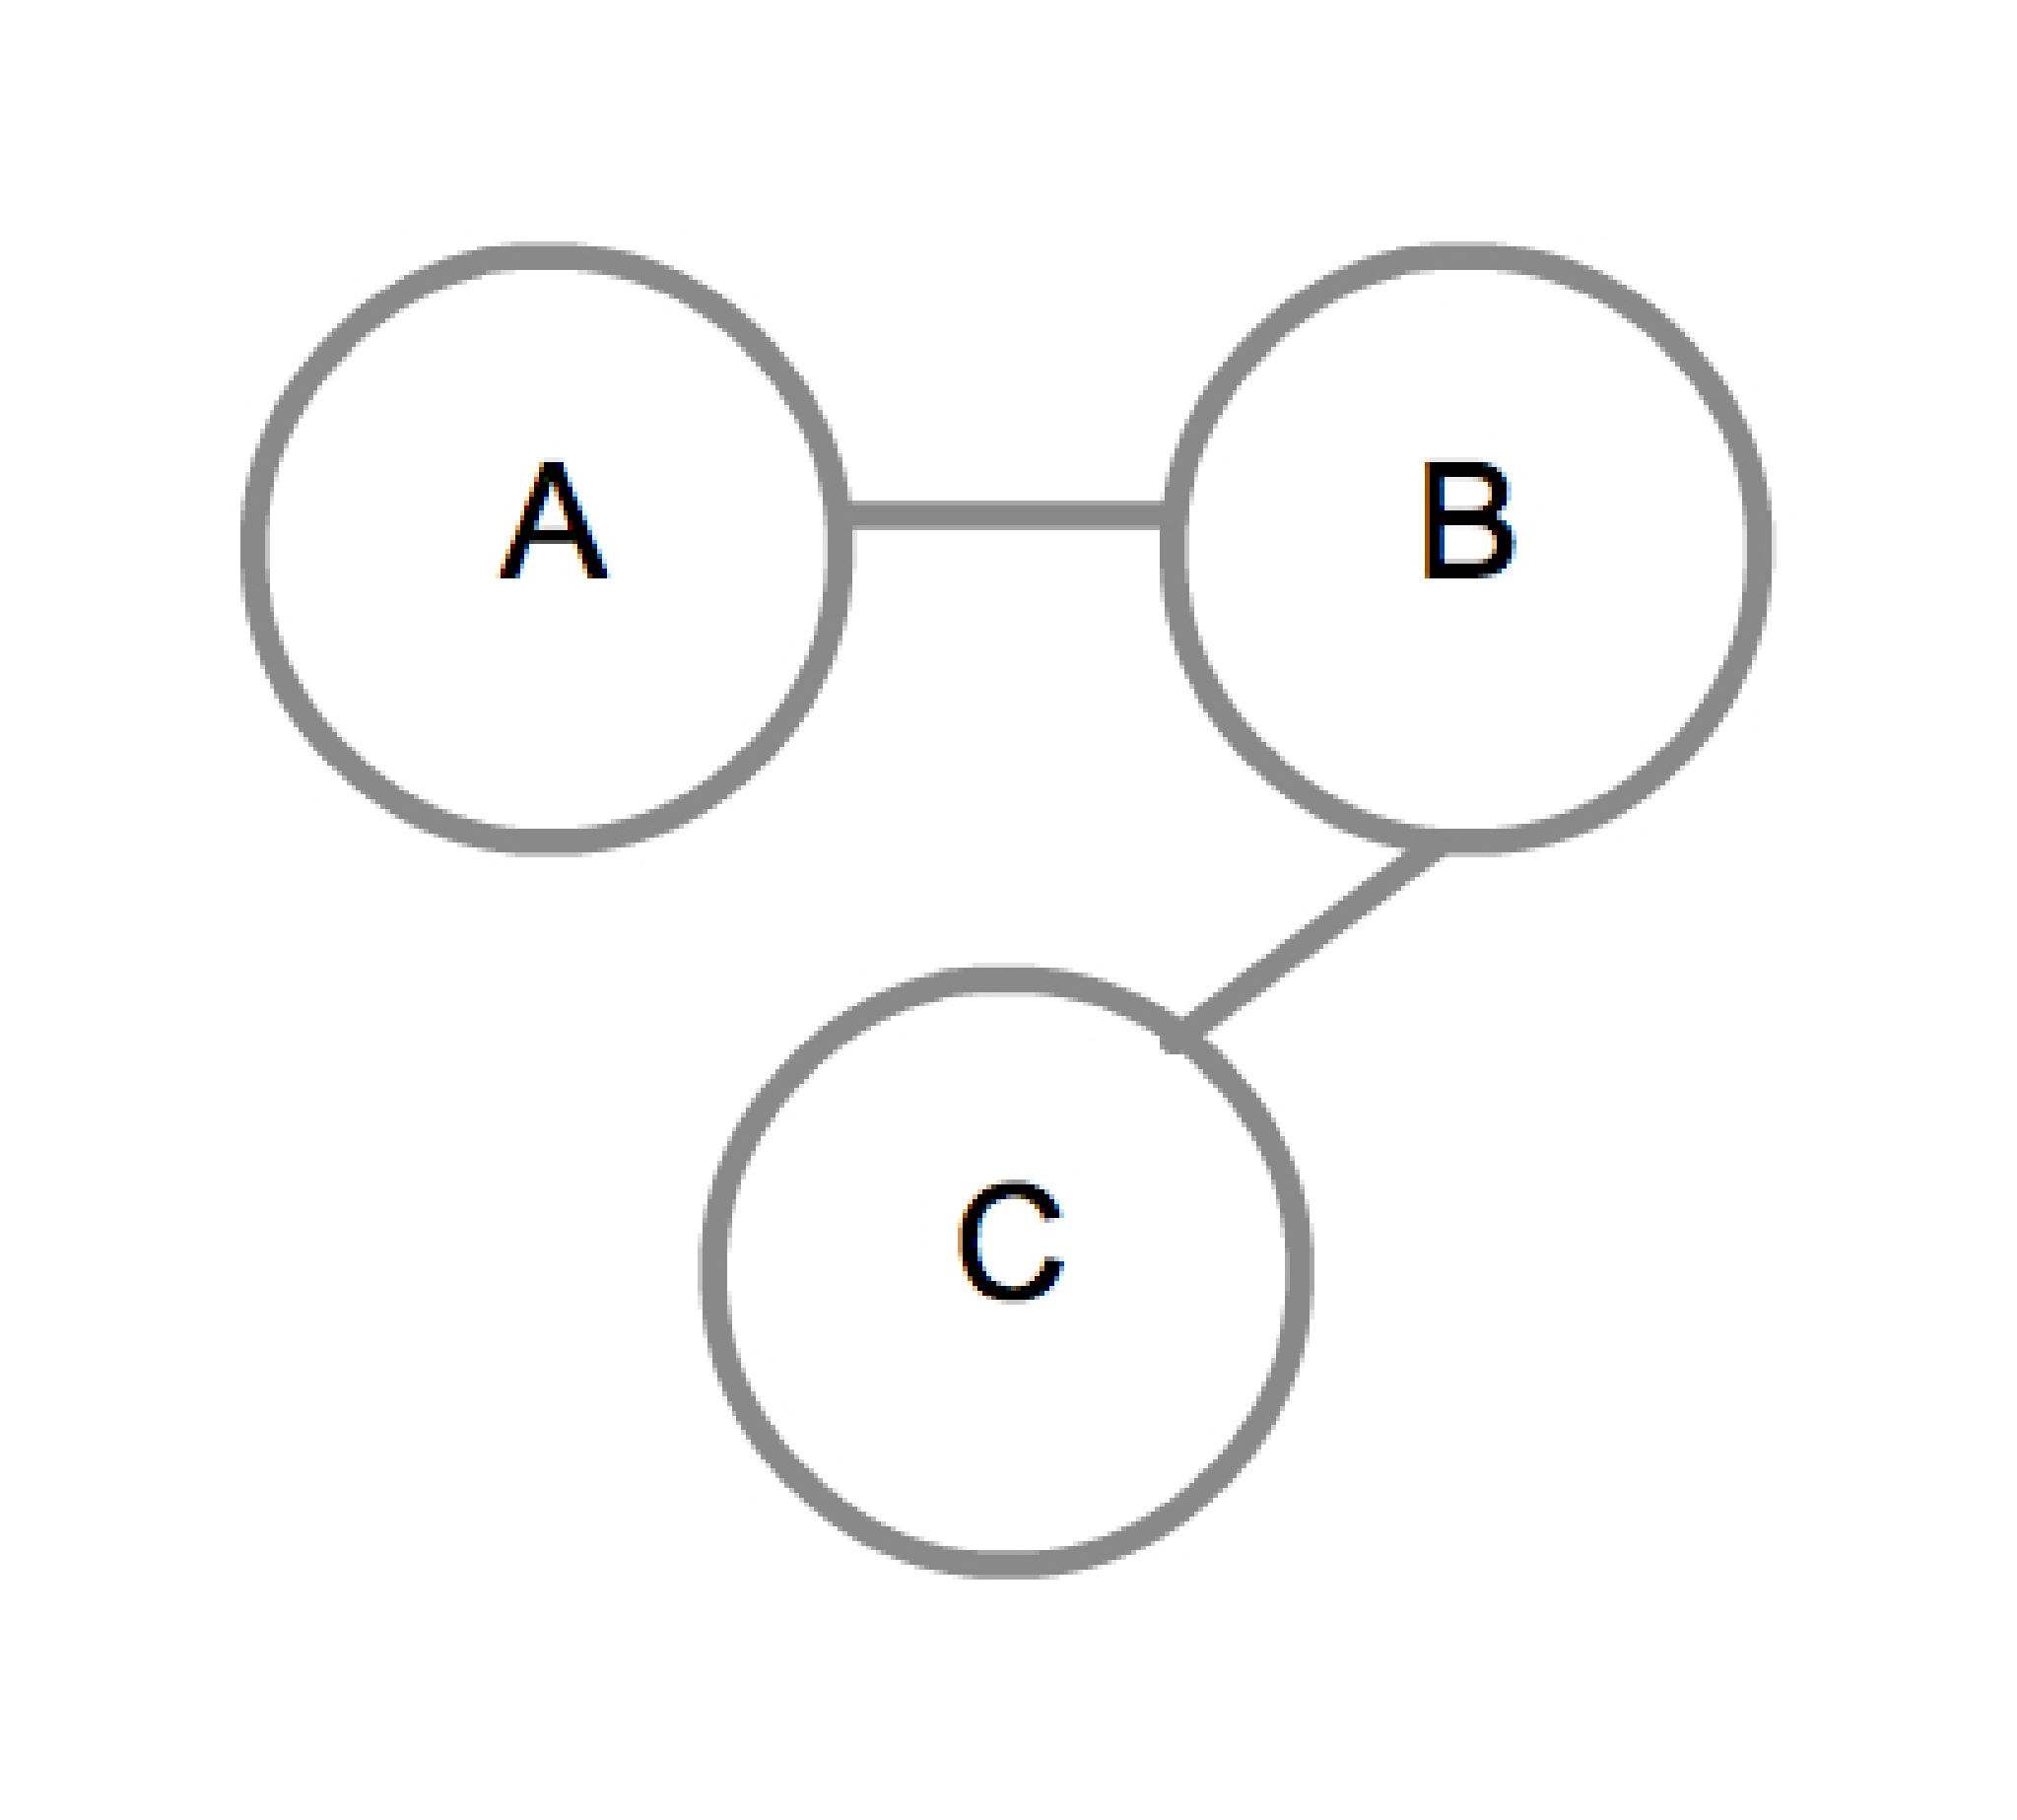
\includegraphics[scale=0.2]{SimpleGraph}
  %\caption{Demonstrates a simple graph}
  \label{fig:SimpleGraph}
}

Note that the vertices are represented by labeled circles and the
edges are represented by lines connecting vertices to one another.

The number of edges connecting a vertex $v$ is called the degree of
$v$ or $deg(v)$.  In the above example:

\begin{align*}
deg(A) = deg(C) &= 1 \\
deg(B) &= 2
\end{align*}

Sometimes an edge is directional, meaning the pair of vertices in an
edge is ordered.  In other words, the edge $(A, B)$ connects $A$ to
$B$, but not $B$ to $A$.  We say such an edge is incoming on $B$ and
outgoing on $A$.  A graph whose edges are ordered pairs is called a
$directed graph$ or $digraph$.

This is represented visually by an edge with an arrow at one end,
indicating the direction:

{
  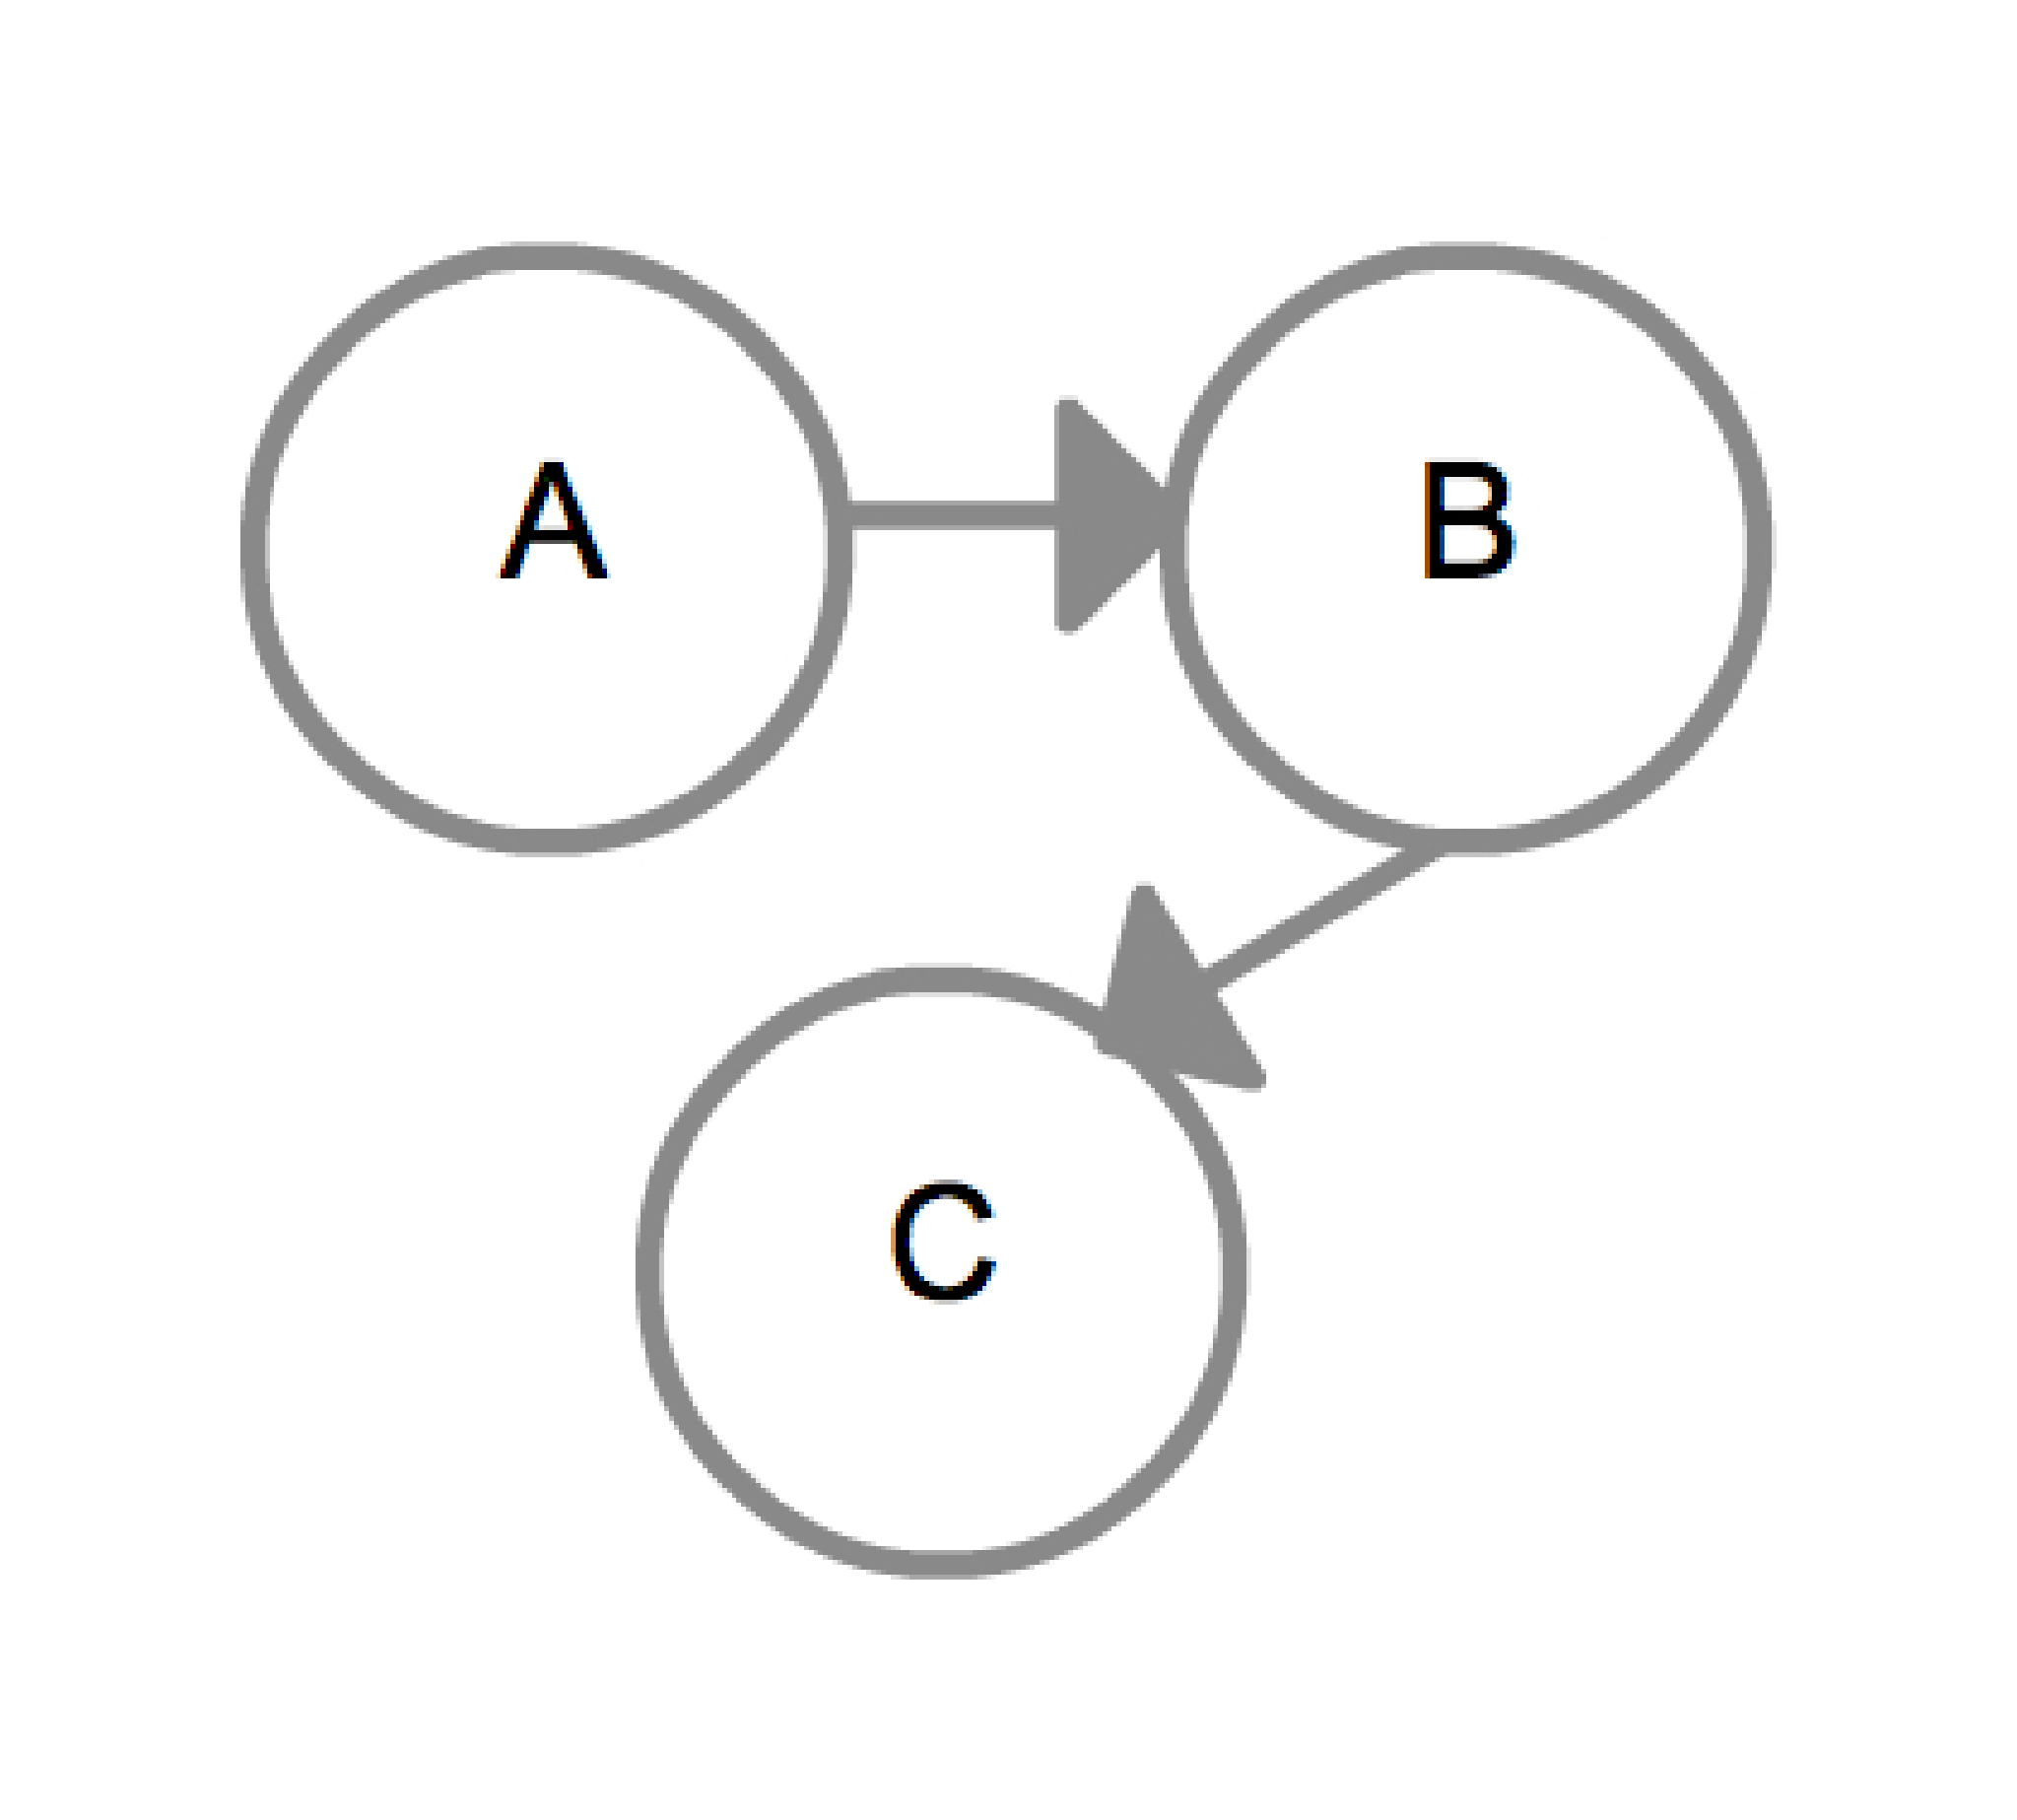
\includegraphics[scale=0.2]{DiGraph}
  %\caption{Demonstrates a directed graph}
  \label{fig:DiGraph}
}

In a digraph, the number of incoming edges of $v$ is the in-degree or
$deg^-(v)$.  Similarly, the number of outgoing edges is the
out-degree or $deg^+(v)$.

In the above example:
%
\begin{align*}
deg^+(A) = deg^+(B) &= 1 \\
deg^-(B) = deg^-(C) &= 1 \\
deg^+(C) = deg^-(A) &= 0
\end{align*}

A \emph{simple graph} is a graph which contains no edges from any
vertex $v$ to itself $ (v,v) $, called loops.  A simple graph also
contains no multi-edges which connect more than two vertices.

A \emph{path} is a sequence of edges from vertex $u$ to vertex $v$.

Two vertices are said to be \emph{connected} if there exists a path
between them.  

A graph is said to be connected if for any two vertices, there exists
a path between them. An adjacent vertex is called a \emph{neighbour}.

A \emph{complete} graph is one in which every vertex is adjacent to
every other vertex.

A \emph{subgraph} is a graph consisting of a subset of the vertices
and edges in another graph.

A \emph{connected component} is a connected subgraph which does
not disconnect any adjacent vertices.  It should be easy to see that a
connected graph has exactly one connected component.

A \emph{cycle} in a graph is when there exists a path from a vertex
back to itself without crossing any edge more than once.

A graph is said to be \emph{acyclic} when it does not contain cycles.

\section{Representation}

\subsection{Adjacency List}

One way to represent a graph is for every vertex, store a list of
neighbours.  For example:

{
  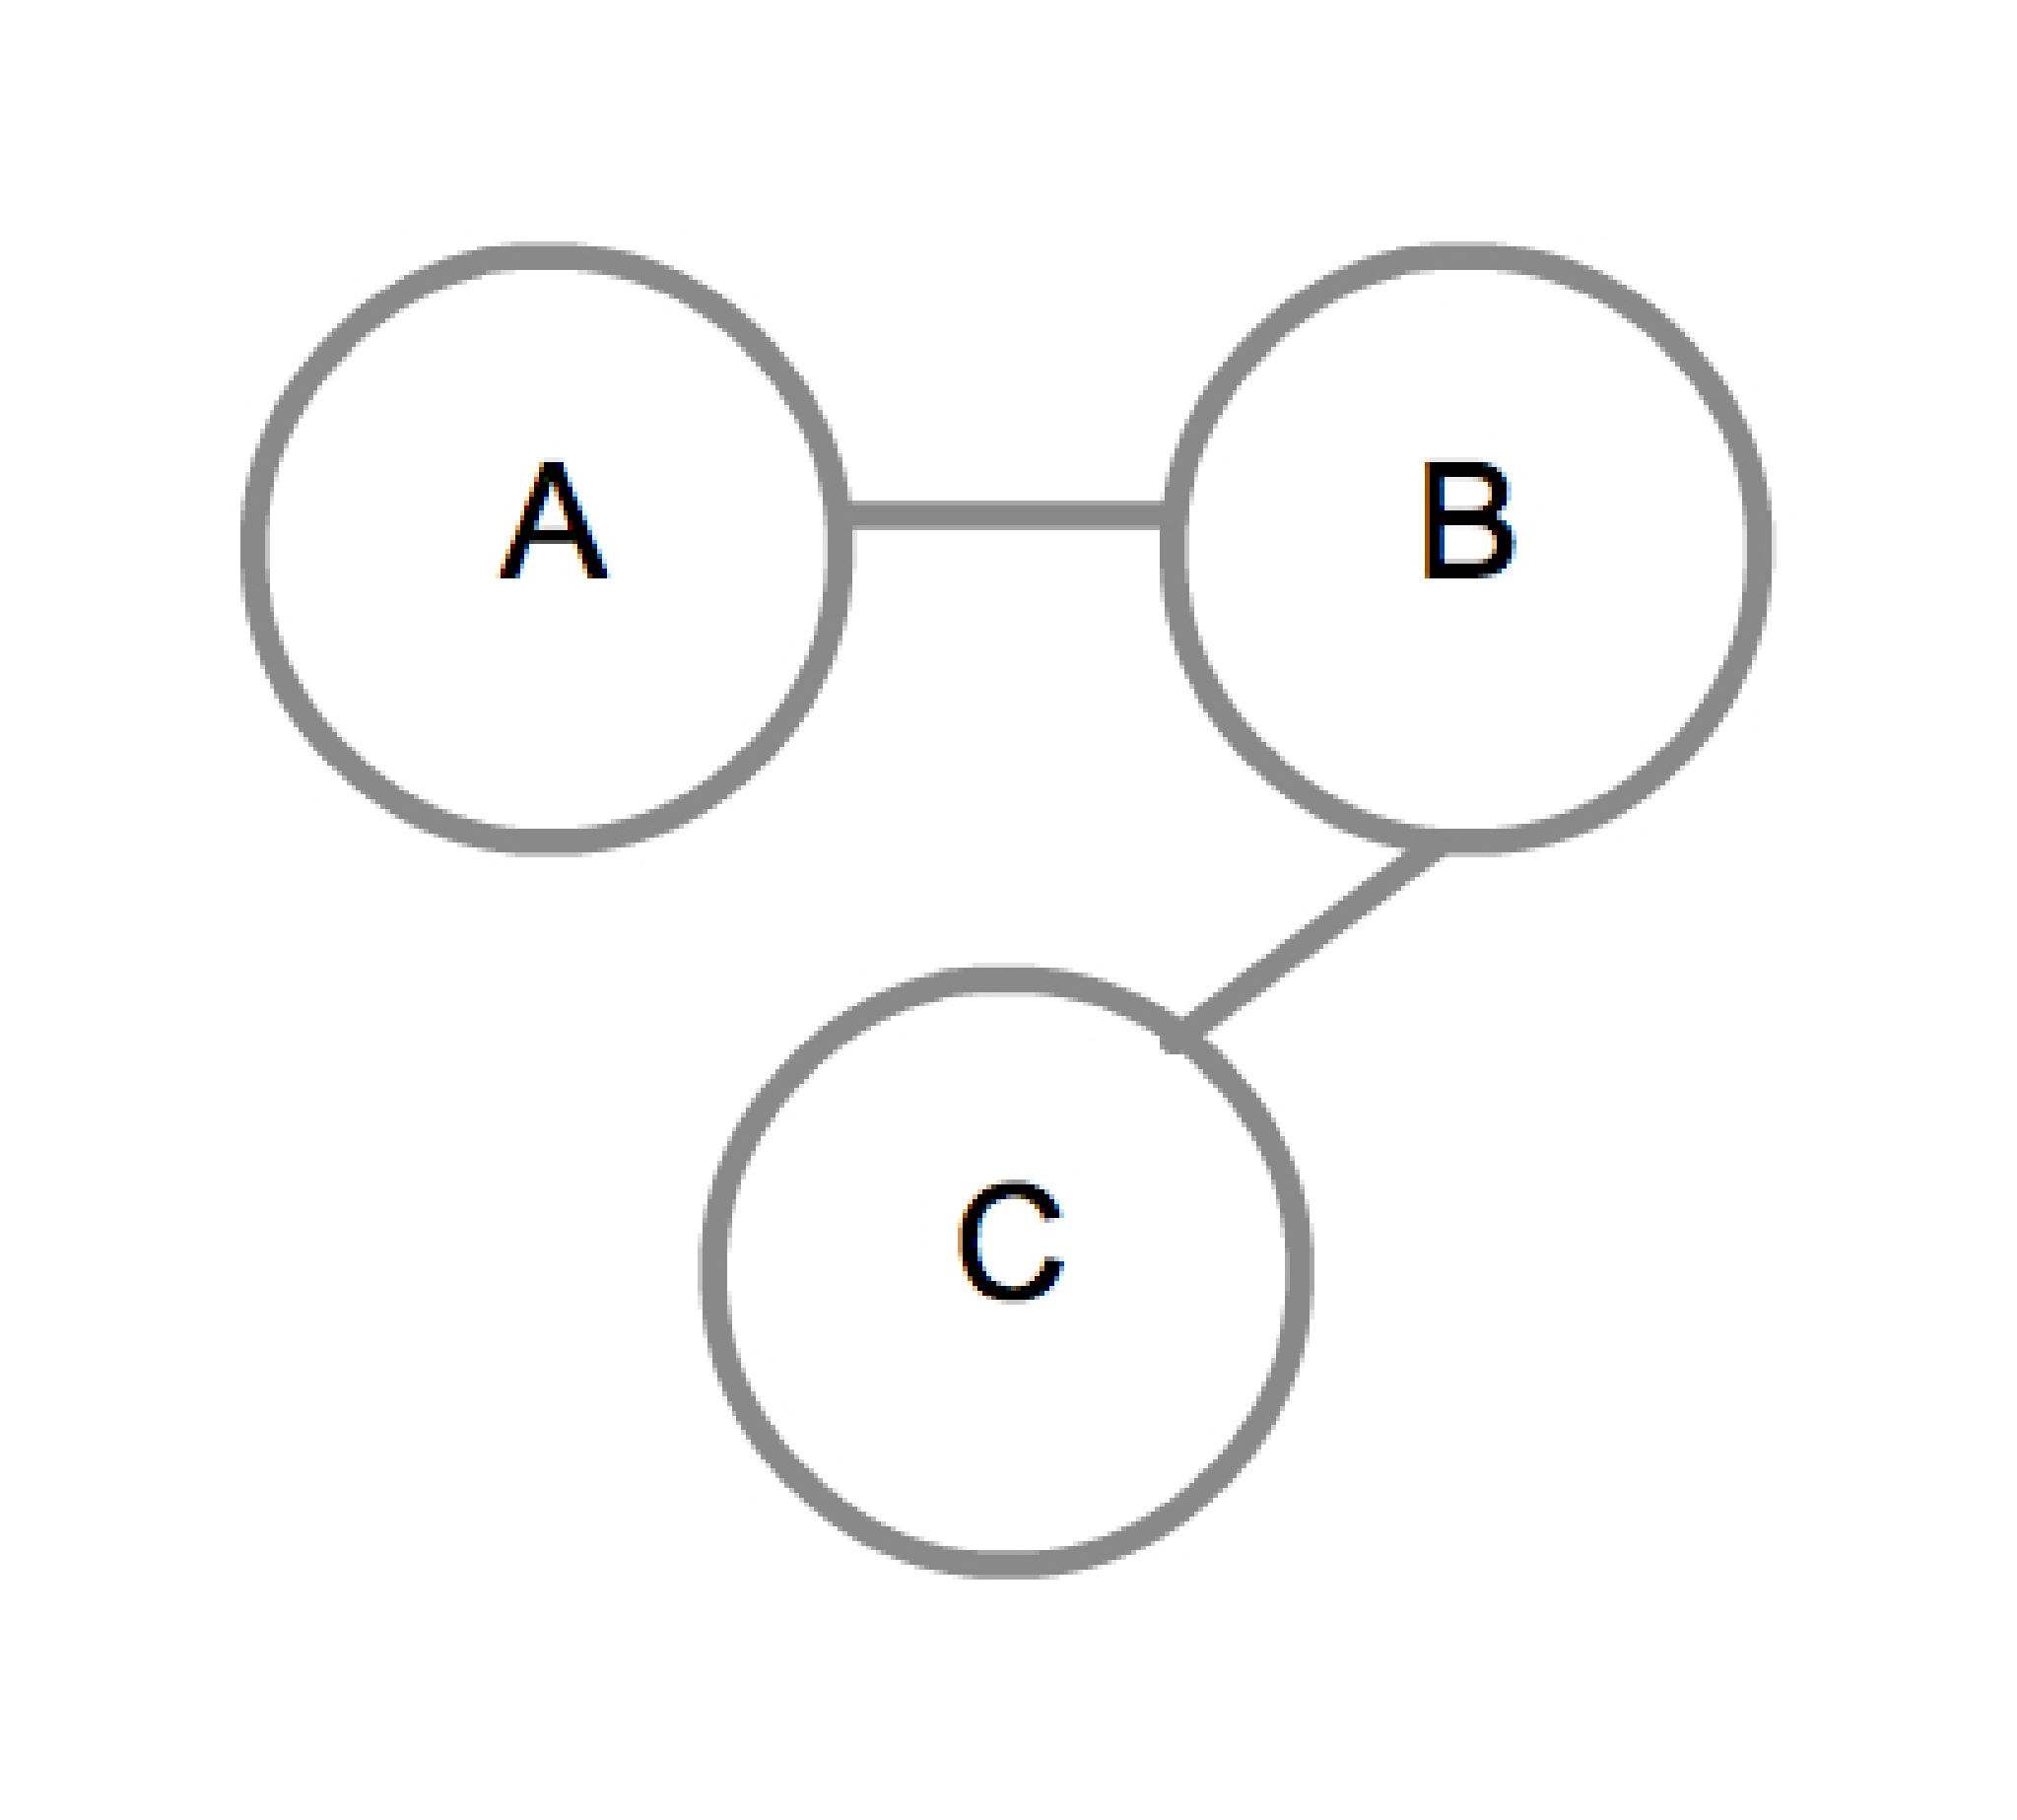
\includegraphics[scale=0.2]{SimpleGraph}
  %\caption{Demonstrates a simple graph}
  \label{fig:SimpleGraph}
}

can be represented:

{
  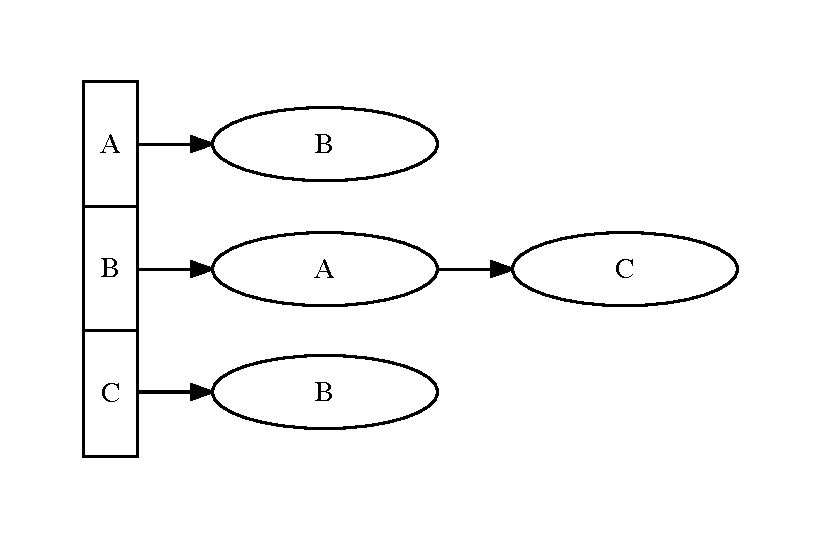
\includegraphics[scale=0.7]{AdjacencyList}
  %\caption{Demonstrates an adjacency list for a simple graph}
  \label{fig:AdjacencyList}
}

And

{
  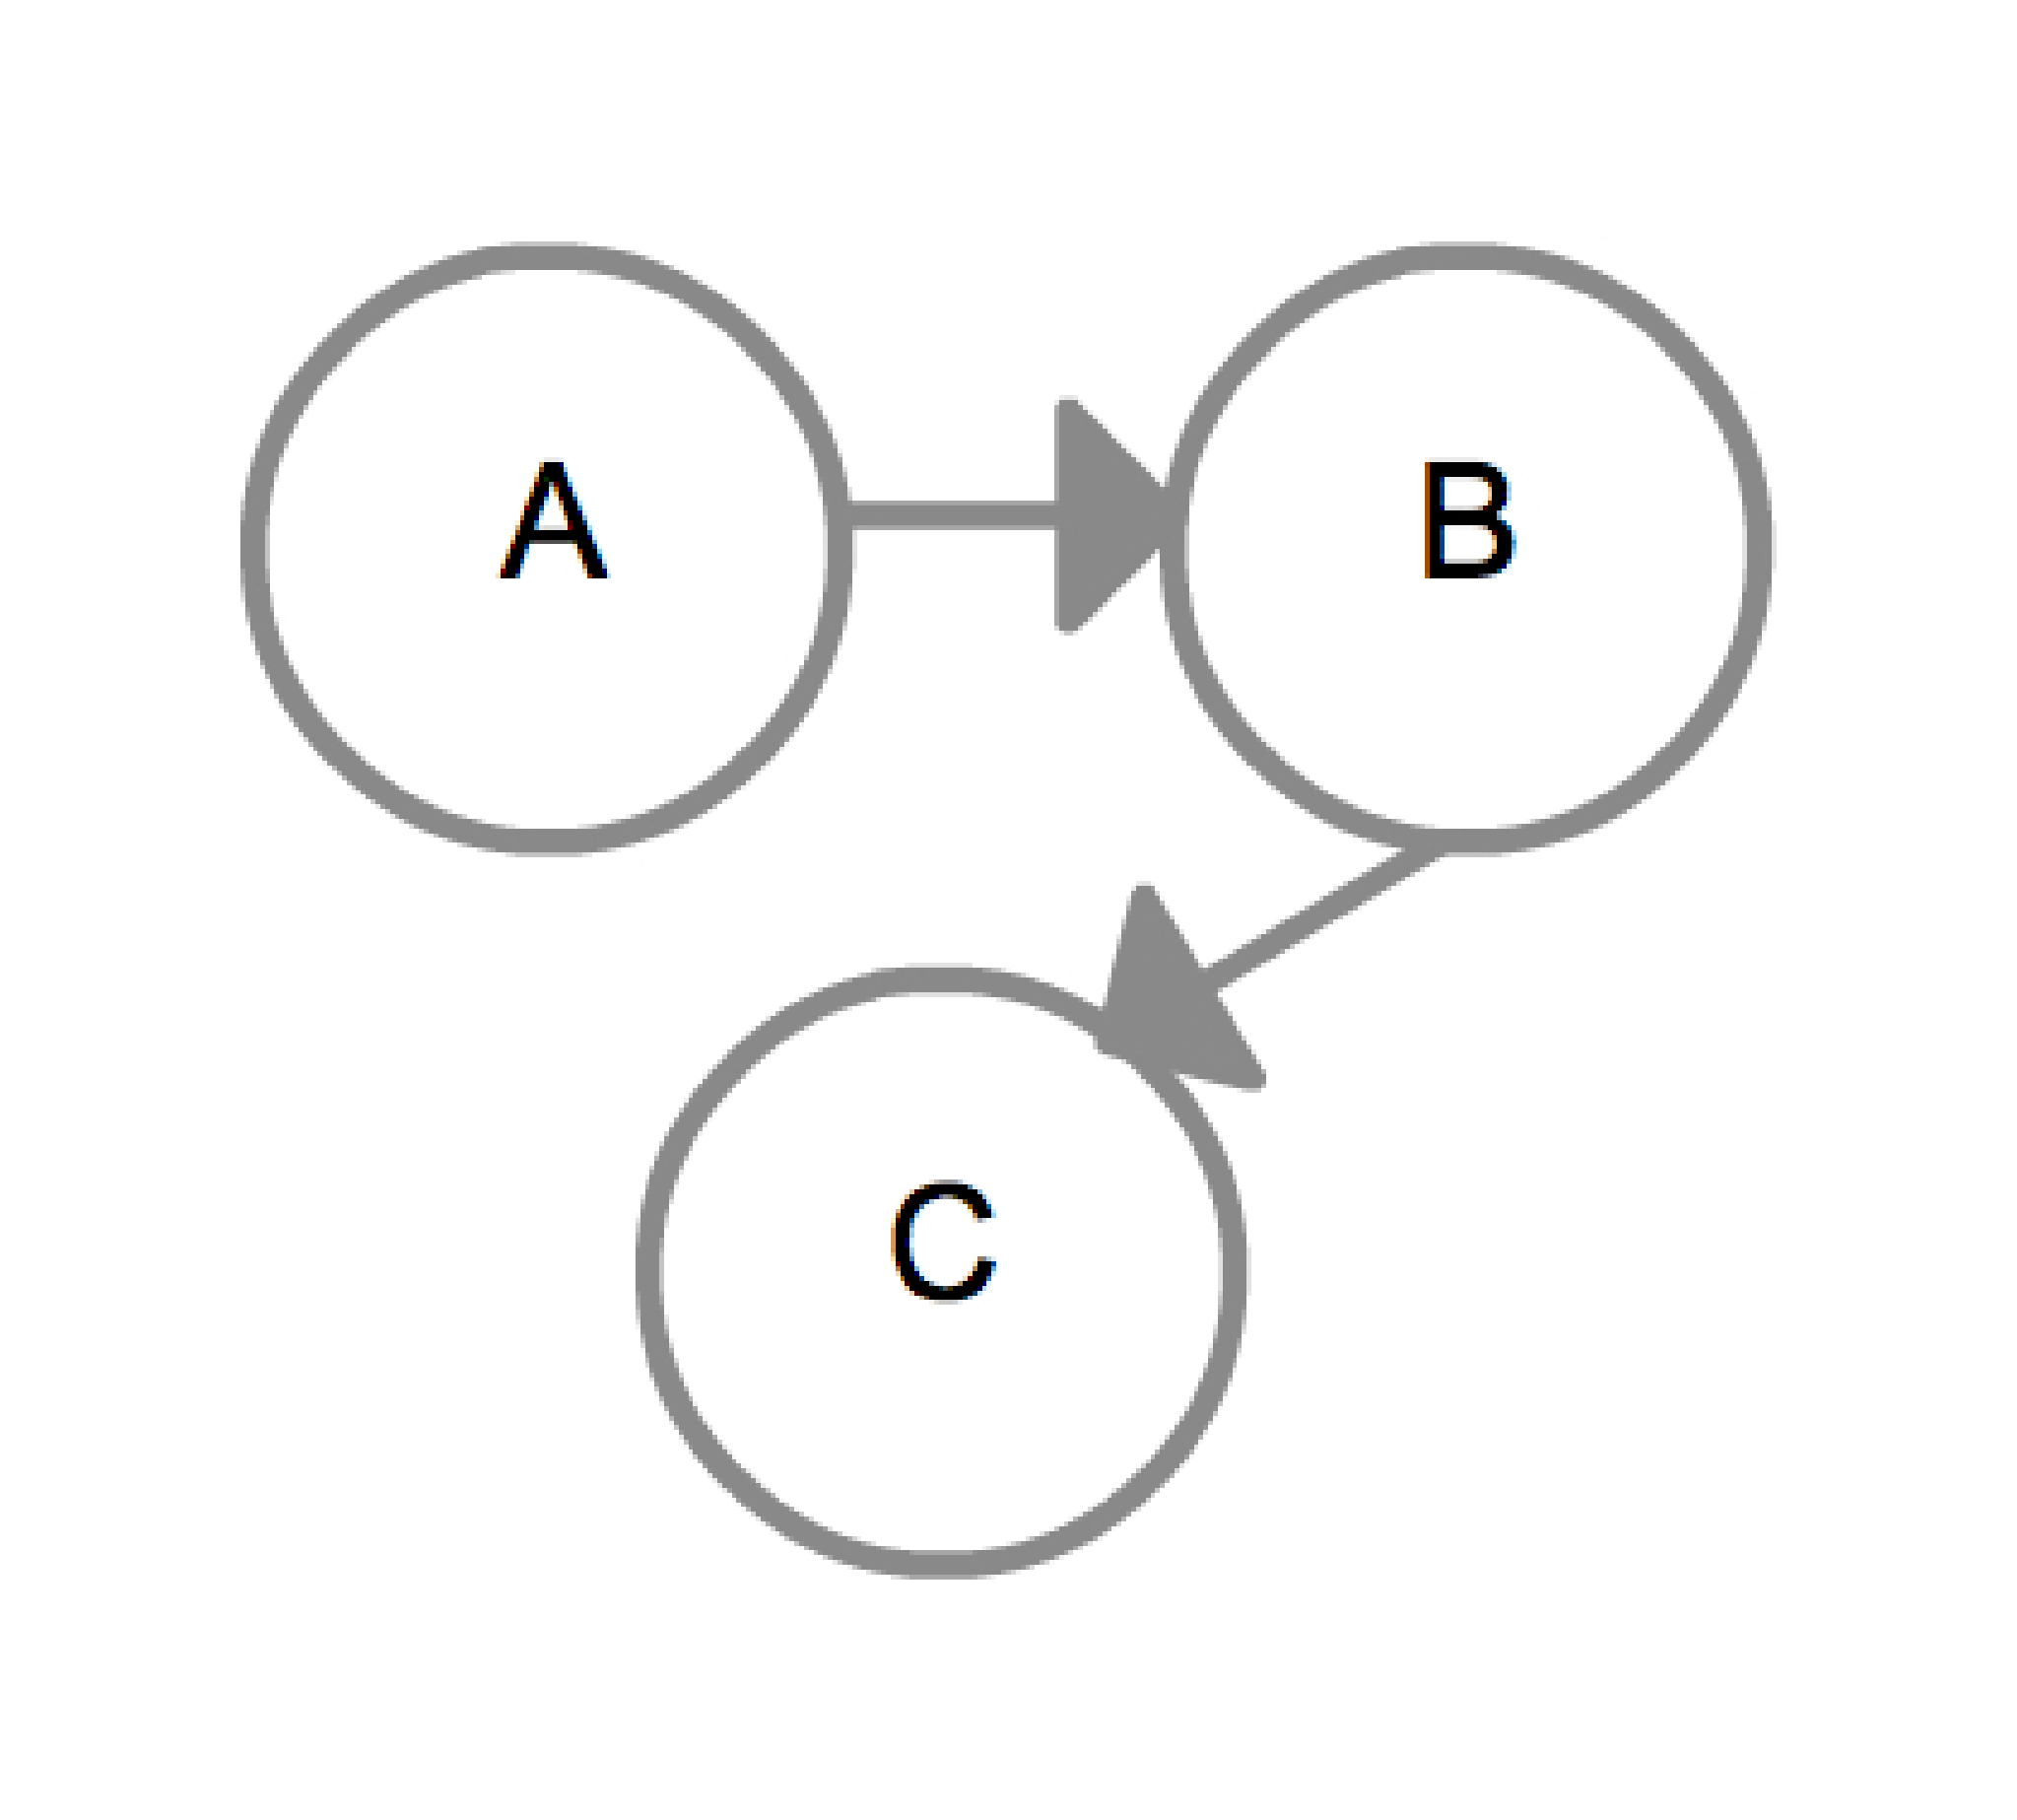
\includegraphics[scale=0.2]{DiGraph}
  %\caption{Demonstrates a directed graph}
  \label{fig:DiGraph}
}

can be represented:

{
  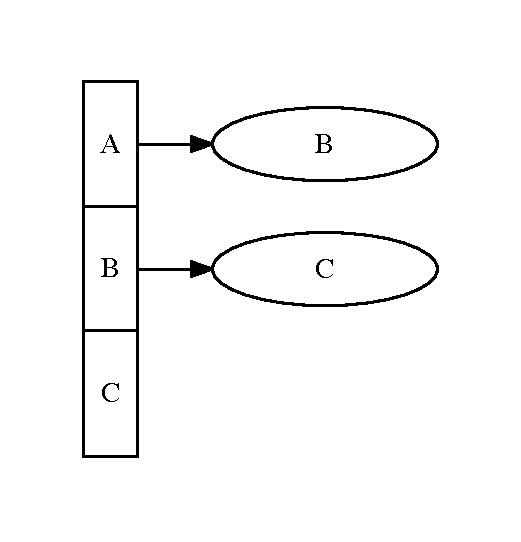
\includegraphics[scale=1.0]{AdjacencyListDigraph}
  %\caption{Demonstrates an adjacency list for a directed graph}
  \label{fig:AdjacencyListDigraph}
}

\subsection{Adjacency Matrix}

Another representation of a graph is as a square matrix with $n$ rows
and columns where the element at row $i$ and column $j$ is 1 if there
is an edge between $v_i$ and $v_j$ and 0 otherwise.  For example:

{
  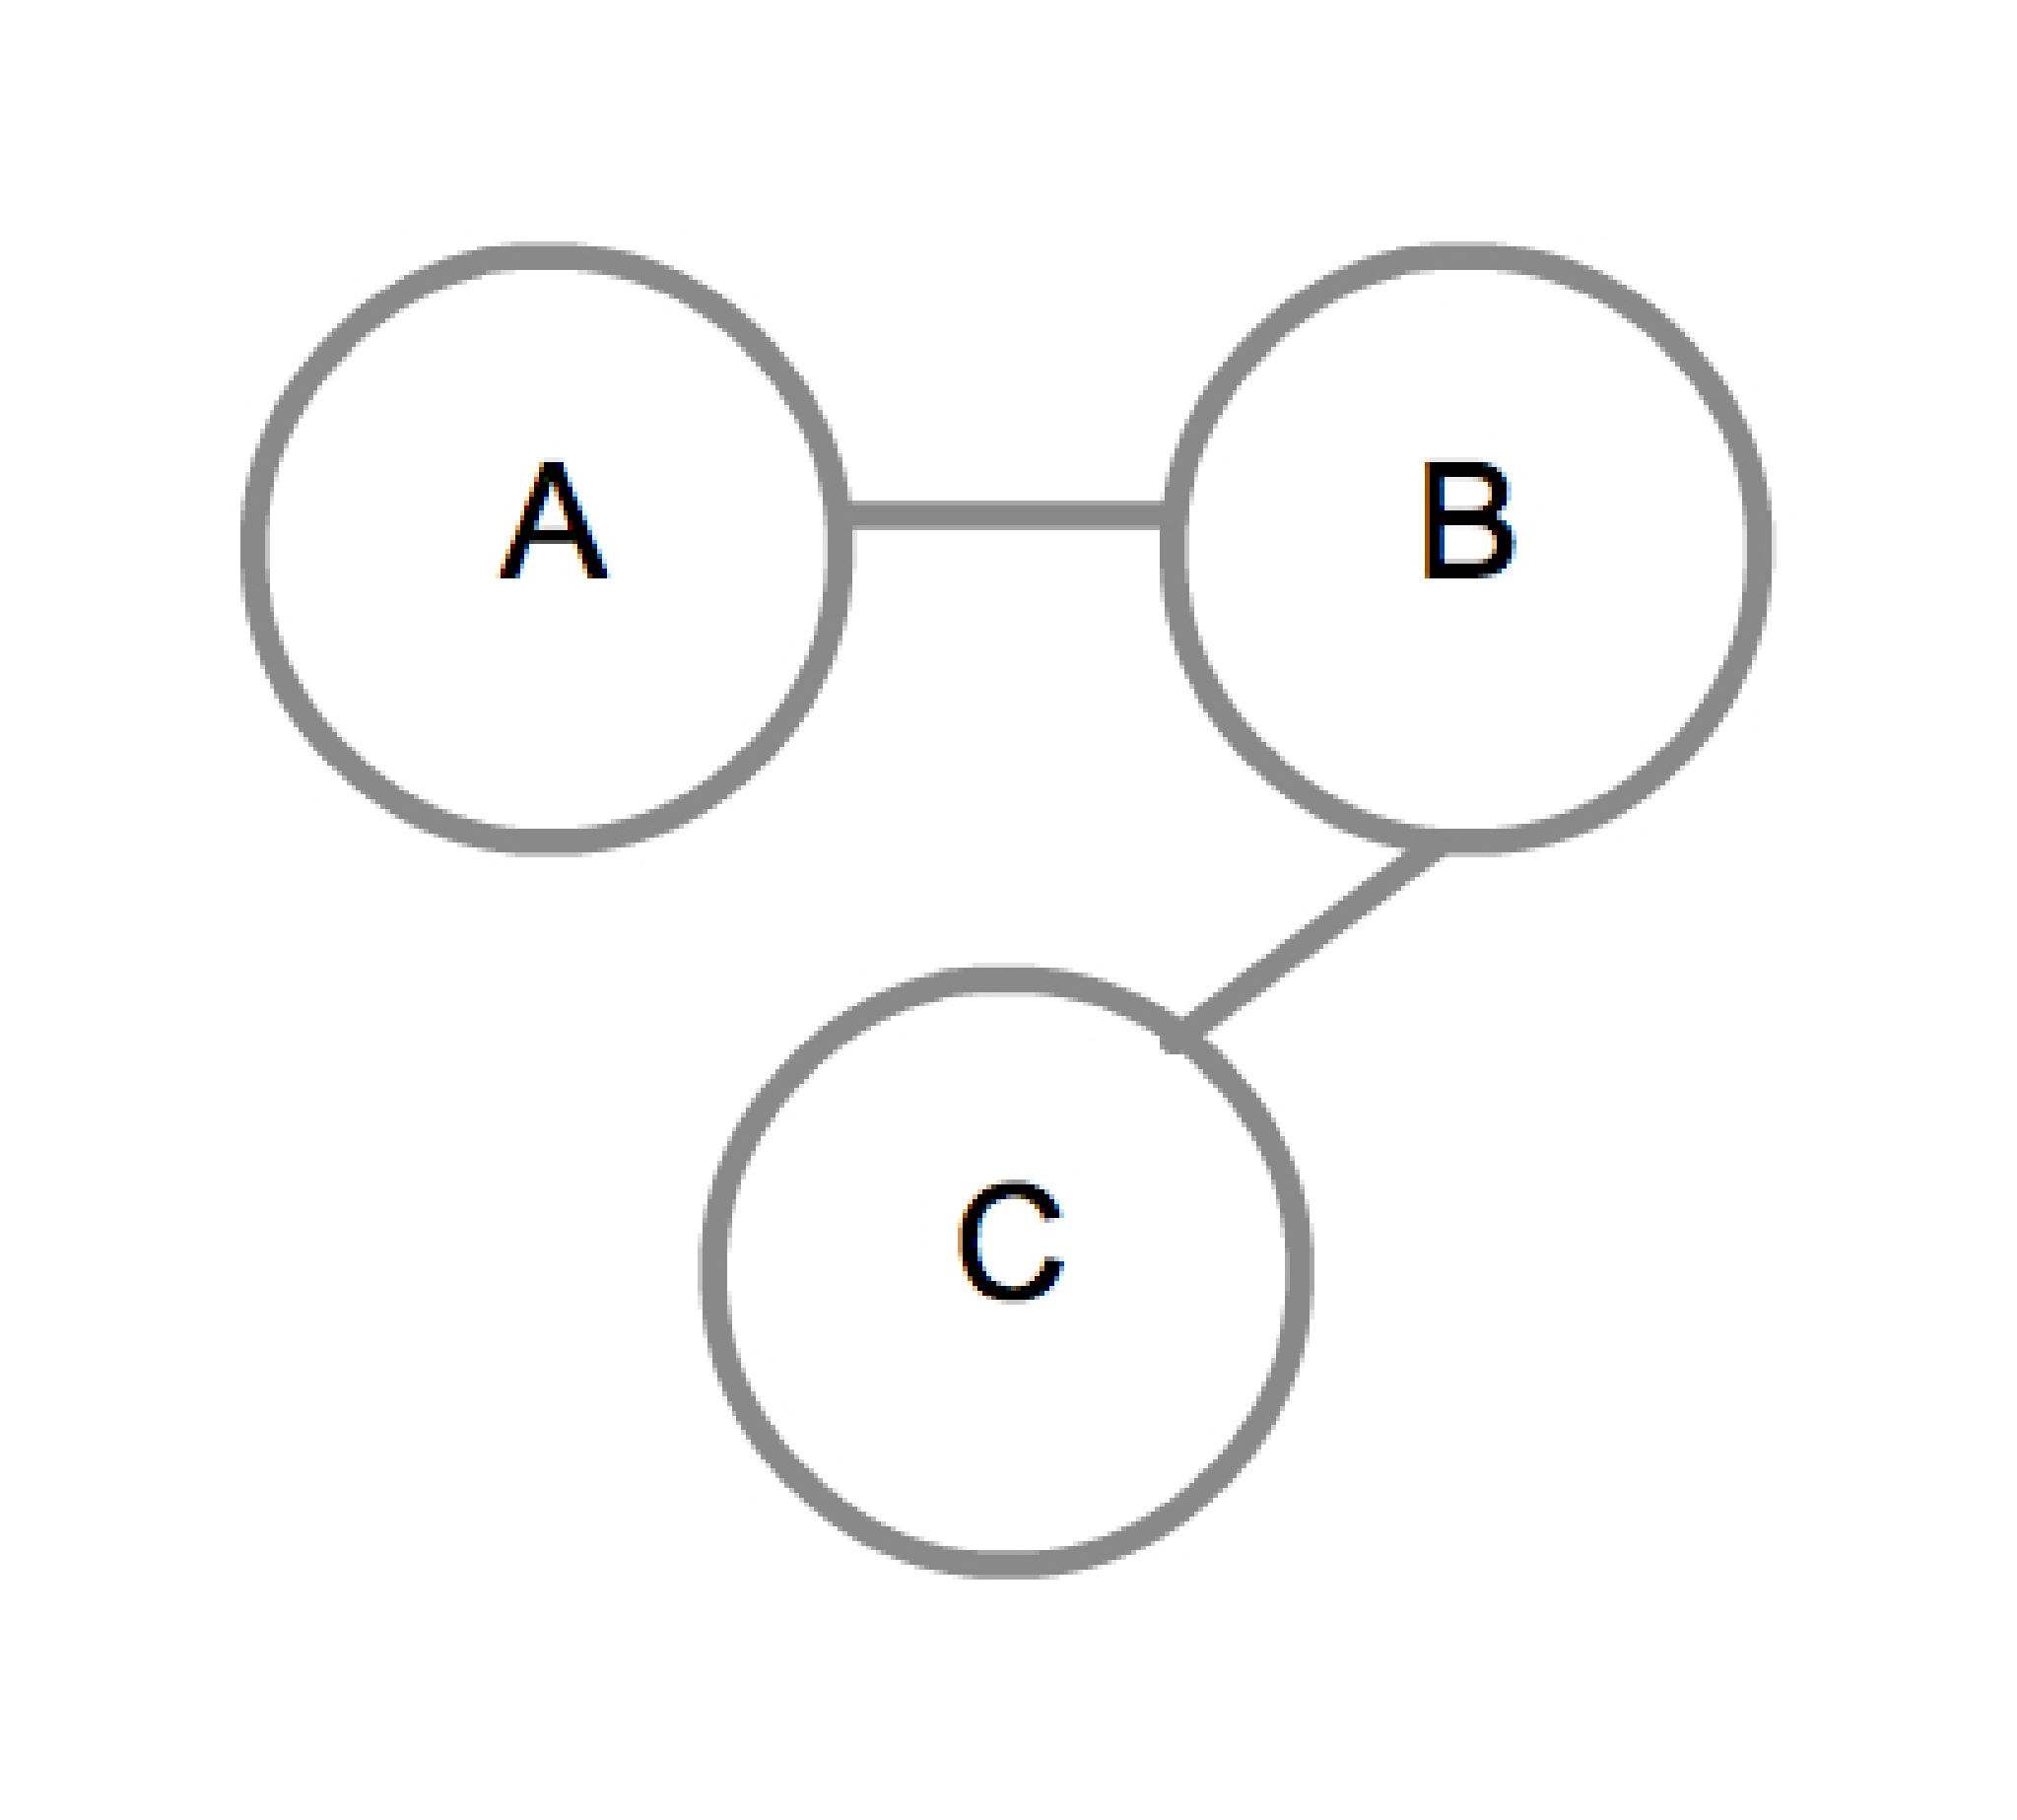
\includegraphics[scale=0.2]{SimpleGraph}
  %\caption{Demonstrates a simple graph}
  \label{fig:SimpleGraph}
}

can be represented

\[
\left[
\begin{array}{cccc}
  & a & b & c \\
a & 0 & 1 & 0 \\
b & 1 & 0 & 1 \\
c & 0 & 1 & 0
\end{array}
\right]
\]

As for directed graphs, row $i$ column $j$ is 1 if there exists an
edge $(v_i,v_j)$.  For example:

{
  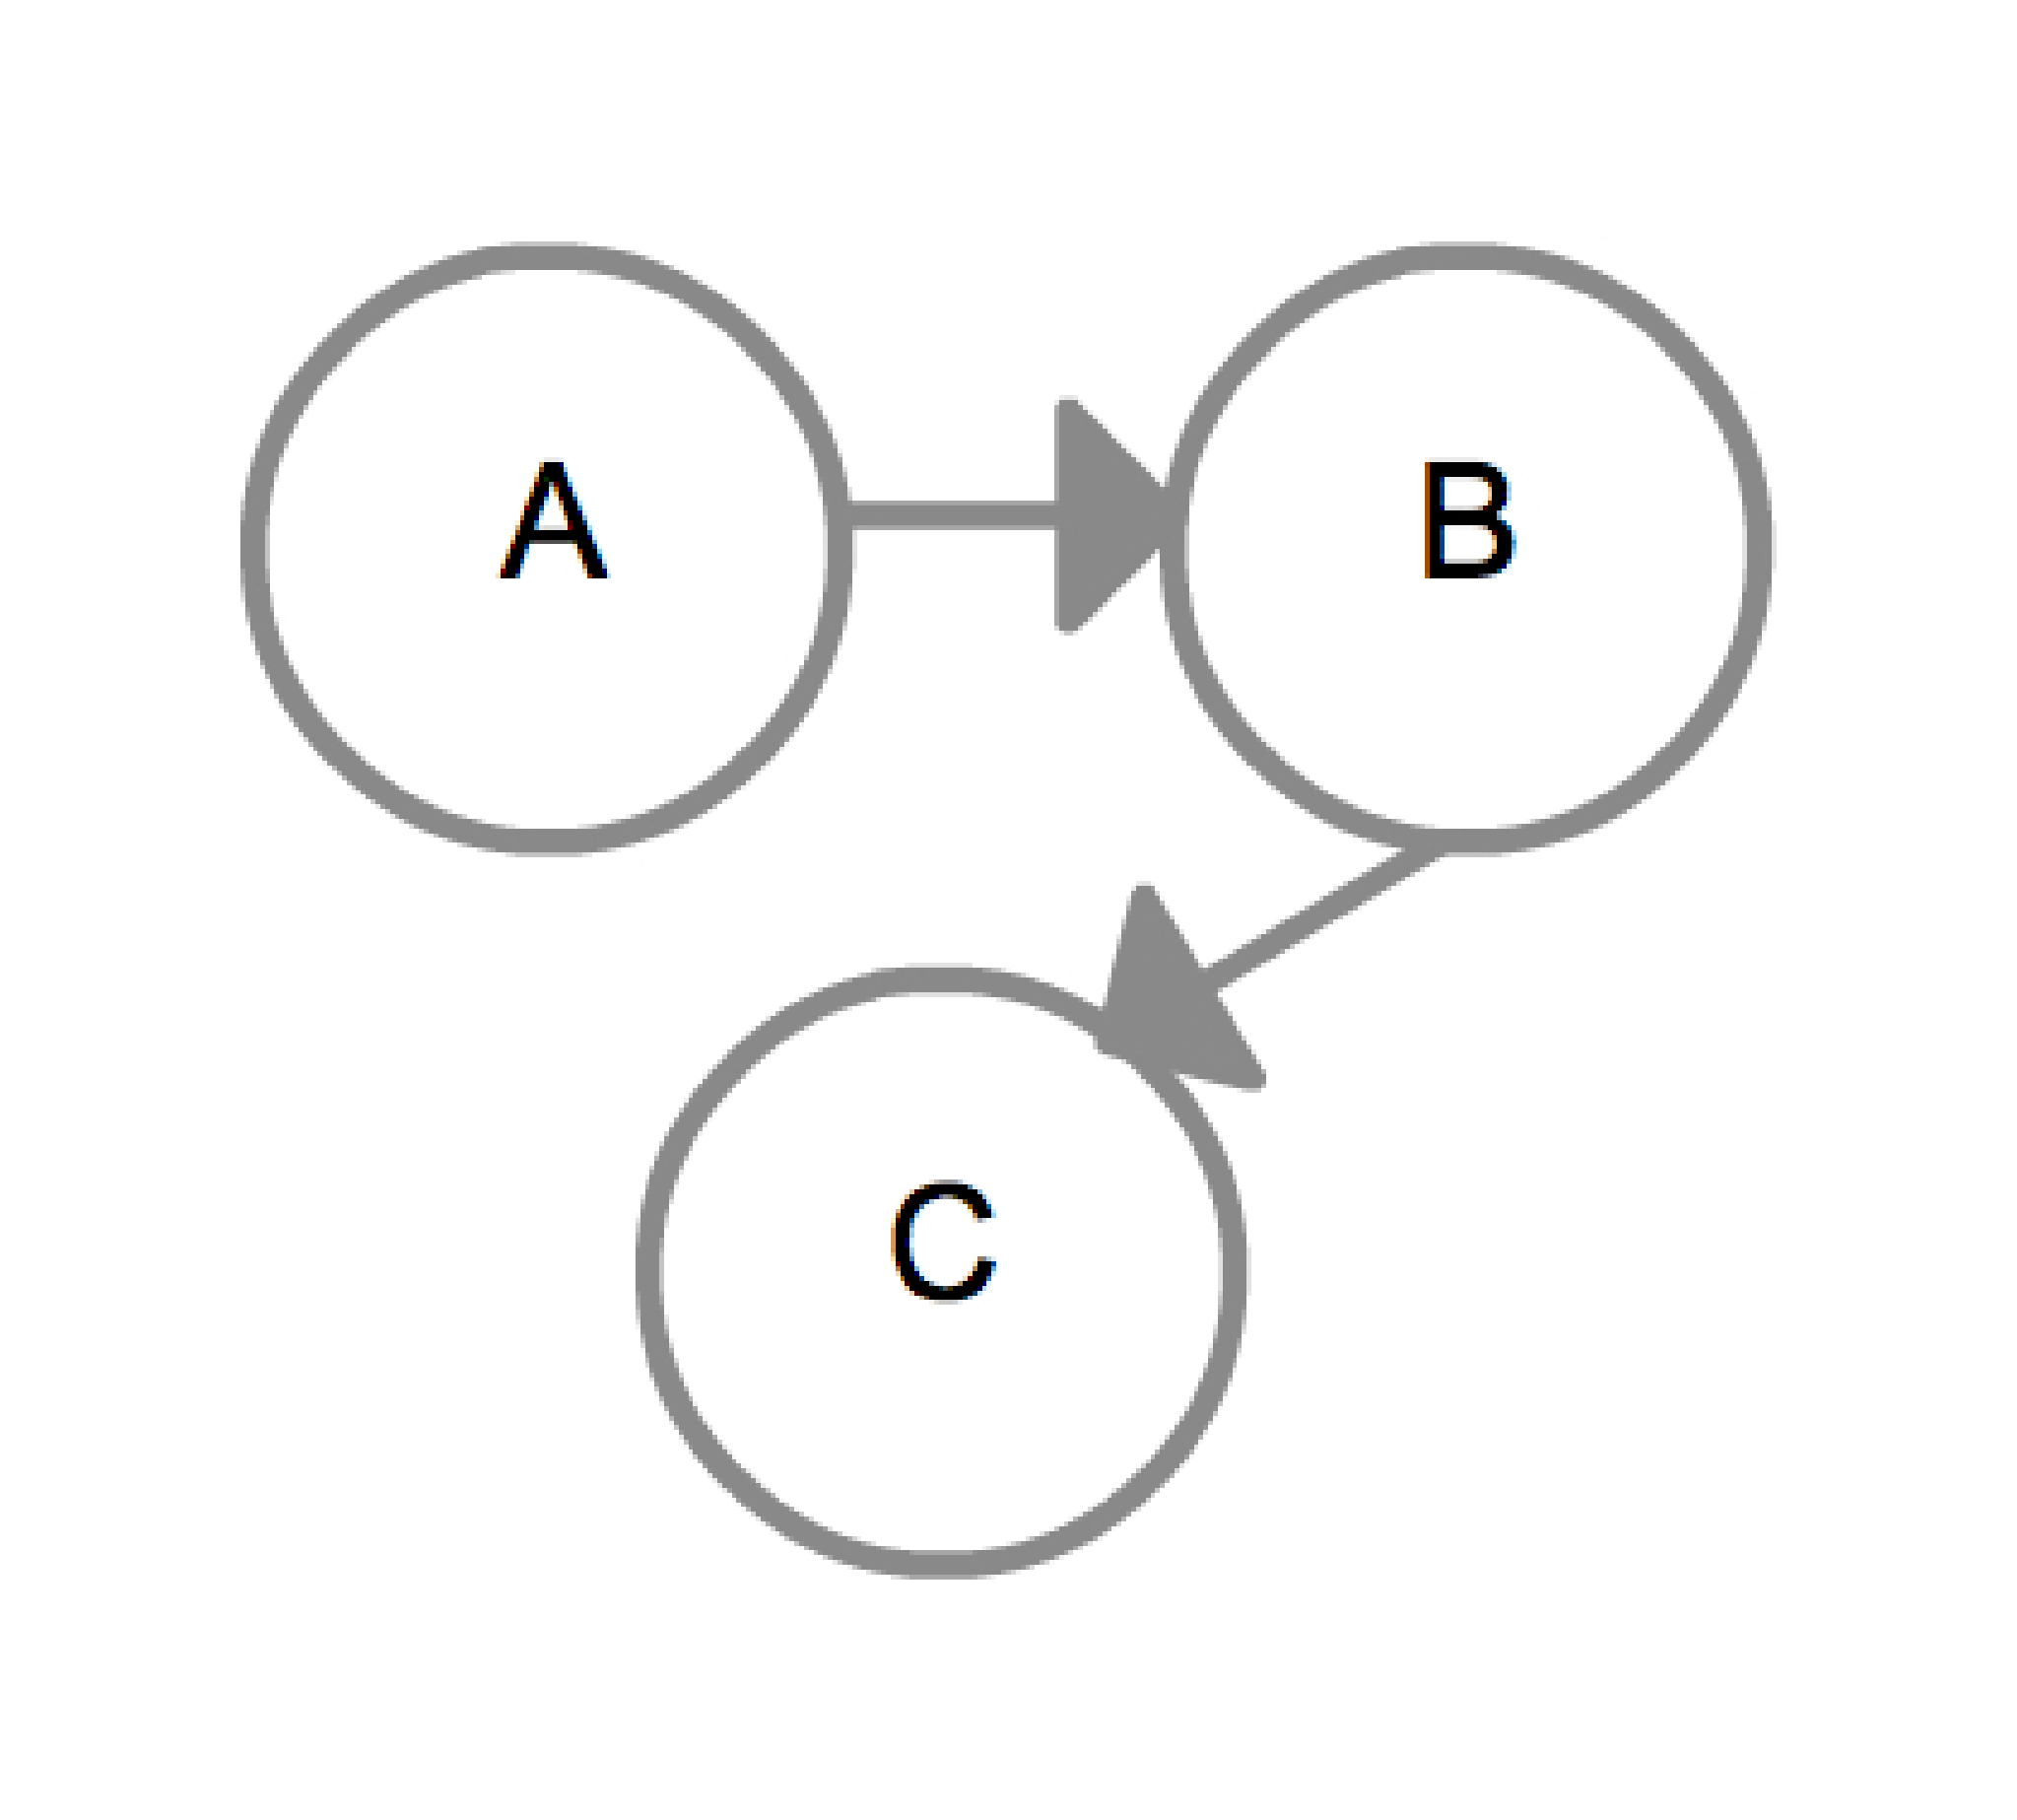
\includegraphics[scale=0.2]{DiGraph}
  %\caption{Demonstrates a directed graph}
  \label{fig:DiGraph}
}

can be represented

\[
\left[
\begin{array}{cccc}
  & a & b & c \\
a & 0 & 1 & 0 \\
b & 0 & 0 & 1 \\
c & 0 & 0 & 0
\end{array}
\right]
\]
                      % done
  \chapter{Depth-First Search}

One important operation in a graph is search.  A useful kind of search
is Depth-First, in which we begin as some start node, marking the node
visited, then we recurse on the neighbours one by one until no more
unvisited neighbours exist.

During a visit, we label each node with a number before visiting its
children and another number after visiting its children.  This number
(called the clock) starts at 1, and is incremented every time a node
receives a label.  The number a node $v$ receives before its children
are visited is called its pre-number ($pre(v)$), and the number that
node receives after its children are visited is called its post-number
($post(v)$).

\begin{theorem}[Parenthesis Theorem]

For nodes $u,v$, the interval between $pre(u)$ and $post(u)$ and the
same interval for $v$ are either:

\begin{itemize}

\item Entirely disjoint
\item The interval of $u$ is completely within the interval of $v$
\item The interval of $v$ is completely within the interval of $u$

\end{itemize}

The name comes from the fact that this is just like properly nested
parentheses.

\end{theorem}

Running a DFS on a graph reveals a tree structure where the start node
is the root and neighbours are parent and child depending on which was
visited first.  There are a few interesting classifications of edges
in a DFS tree:

\begin{enumerate}

\item A \emph{Tree Edge} goes from a parent node to a child node.

\item A \emph{Forward Edge} goes from ancestor to descendant (but not
  parent to child)

\item A \emph{Back Edge} goes from descendant to ancestor

\item A \emph{Cross Edge} goes to a non-ancestor non-descendant

\end{enumerate}
\begin{center}
\begin{tikzpicture}[>=latex,scale=1.5]
    \SetUpEdge[lw           = 1.0pt,
               labelstyle   = {draw,sloped}]
    \SetGraphUnit{1}
    \GraphInit[vstyle=Normal] 
    \tikzset{VertexStyle/.style = {
    shape = circle,
    inner sep = 0pt,
    outer sep = 0pt,
    minimum size = 6pt,
    draw}}
    \Vertex{G}
    \NOEA(G){B}
    \SOEA(G){F}
    \EA(B){A}
    \SOEA(A){C}
    \SO(C){D}
    \NO(F){E}
    \tikzset{EdgeStyle/.style={->}}
    \Edge[label=Cross,labelstyle={above,sloped,font=\tiny\bfseries}](C)(B)
    \Edge[label=Tree,labelstyle={above,sloped,font=\tiny\bfseries}](A)(B)
    \Edge[label=Tree,labelstyle={above,sloped,font=\tiny\bfseries}](A)(C)
    \Edge[label=Tree,labelstyle={above,sloped,font=\tiny\bfseries}](B)(E)
    \Edge[label=Tree,labelstyle={above,sloped,font=\tiny\bfseries}](E)(G)
    \Edge[label=Tree,labelstyle={below,sloped,font=\tiny\bfseries}](B)(G)
    \Edge[label=Tree,labelstyle={above,sloped,font=\tiny\bfseries}](G)(F)
    \Edge[label=Tree,labelstyle={above,sloped,font=\tiny\bfseries}](C)(D)
    \Edge[label=Cross,labelstyle={above,sloped,font=\tiny\bfseries}](D)(F)
    \tikzset{EdgeStyle/.style={->,relative=false,in=150,out=100}}
    \Edge[label=Forward,labelstyle={above,sloped,font=\tiny\bfseries}](A)(G)
    \tikzset{EdgeStyle/.style={->,relative=false,in=0,out=0}}
    \Edge[label=Back,labelstyle={above,sloped,font=\tiny\bfseries}](D)(A)
\end{tikzpicture}
\end{center}

\begin{theorem}
A digraph has a cycle if and only if a DFS reveals a back edge.
\end{theorem}

\begin{proof}

First let us assume there is a back edge.  By definition this is a
descendant linking back to an ancestor, which has already been
visited.  This gives us a cycle.

Next let us assume there is a cycle.  A DFS will visit each node in
the cycle, and as soon as the last edge in the cycle is visited it
will link a descendant to ancestor which is the definition of a back
edge.

\end{proof}

\begin{theorem}

After running a DFS on a directed acyclic graph (DAG), each edge leads
to a vertex with a lower post number.

\end{theorem}

The proof of this theorem is left up to the reader.
                         % done
  \chapter{Minimum Spanning Tree}

Given an undirected, connected graph where each edge has positive
weight, the \emph{Minimum Spanning Tree} (MST) is a connected subgraph on the same 
vertex set with minimal weight. Intuitively, the MST is the lightest possible
connected subgraph. The MST is not necessarily unique, 
for proof of this, consider a graph where all edges are of equal weight. 
Any tree is an MST of such a graph. 

\section{Kruskal's Algorithm}

%The idea of this algorithm is to begin with the vertex list and an
%empty edge list, and maintain a forest, adding the edge of minimum
%weight that does not make a cycle until the forests are connected.

Kruskal's algorithm for computing the MST relies on the simple observation
that the smallest edge in a graph $G$ is part of \emph{some} MST of $G$.
Kruskal's algorithm starts by constructing a min-heap containing all $m$ edges
in $G$, and a collection of disjoint sets, each containing one of the
$n$ vertices of $G$. We also construct an empty list $T$ that will hold
all the edges of the MST. We then get the minimum edge from the heap, check if
the two nodes the edge joins are from the same set, and if not add 
the edge to $T$, and $union$ the two sets that the edge joins.
We repeat this until $T$ contains $n-1$ edges. 

Because this algorithm uses
structures we already know and understand, analysis will be fairly easy.
We require $O(m) + O(n)$ time to construct the initial sets and heap. We also
require $O(m \log m)$ to extract the minimums from the heap. Our $n-1$ unions
and $n-1$ finds can be done in $(n \log n + n)$ time. Therefore this algorithm
takes $O(m \log m + n \log n)$.

\section{Prim's Algorithm}
Prim's algorithm for computing the MST is fairly similar to Kruskal's. However,
instead of working with all of the edges and vertices at once, it picks one
vertice and builds from that. We start by constructing an empty list $A$ which
will hold all the vertices that are part of the MST so far, a list $T$ which
will hold all the edges in the MST so far, a min-heap $V$ which will contain all
the vertices not in $A$. At first every node is given a key of infinity. 
We then pick a random vertex $v$ from $V$ and move it from $V$ 
to $A$. Next we look at all the edges of $v$ and set the
keys of the corresponding nodes to the weight of these edges. Now we retrieve
the minimum node $u$ from $V$ and move it to $A$, and its key edge to $T$. 
Next we look at all the edges on $u$ and if their weight is smaller than
the current key of their corresponding edge, set the key to that weight. Then
we simply retrieve another node from the heap and repeat. After $n-1$ iterations
we will have a complete MST.

This algorithm requires $O(n)$ time to construct the initial heap and 
initialize the first node, and since we must update at most $m$ keys in the
heap of $n$ elements, it requires $O(m \log n)$ time to do this. Therefore the
entire algorithm takes $O(n + m \log n)$ time.

                         % done
  \chapter{Shortest Path}

Given a weighted graph, one interesting problem is to find the
path with minimal weight.

\section{Single Source}

This instance of the shortest path problem begins at a specific vertex
in the graph, hence ``Single Source.''

\subsection{Dijkstra's Algorithm}

Given an acyclic graph $G=(V,E)$ in which every edge has a positive
weight and a single vertex $s$ from which to start the path, we begin
by labeling all vertices $u \in E | weight(u) = \infty$, then label
$weight(s) = 0$.  We also create a min-heap of the vertices using
weight as key.

We pop-best a vertex $v$ from our heap.  For each edge $e$ incident to
$v$ and some other vertex $u$, we check if $weight(v) + weight(e)$ is
less than $weight(u)$, in which case we set $weight(u) = weight(v) +
weight(e)$ and decrease the key of $u$ in our heap.  We continue this
process until no vertices remain in the heap.

It should be easy to see that if we have a particular target vertex,
we can halt the algorithm as soon as our target is the root of the
heap, because we have found the shortest path to it.

\subsection{Analysis of Dijkstra's Algorithm}

Intuitively, this algorithm has an upper bound of $O(|V|)$ times
however long it takes us to extract the minimum vertex from our heap,
plus $O(|E|)$ times however long it takes us to decrease the key,
since we have to check every vertex and we may have to check every
edge.  Using a standard heap, this gives us $O(|V|log|V| +
|E|log|V|)$.

\section{All Sources}

This instance of the shortest path problem is concerned with several
sources, in which case Dijkstra's Algorithm does not suffice.

\subsection{Floyd-Warshall Algorithm}

The Floyd-Warshall Algorithm is
\hyperlink{sec:floyd_warshall}{discussed in detail in the chapter on
  Dynamic Programming}.

\section{Arbitrary Weights}

A keen reader will have noticed that both Dijkstra's and Floyd
Warshall Algorithms assume positive edge weights.  Neither of which
are generally useful when there may be edges of negative weight.

\subsection{Bellman-Ford Algorithm}

The Bellman-Ford Algorithm can be applied with edges of arbitrary
weight.  Note that even Bellman-Ford doesn't deal with cycles of
negative weight, since these can be used to make any path have an
arbitrarily small total weight.

The Bellman-Ford Algorithm is beyond the scope of these notes, for
more information please see
\href{https://en.wikipedia.org/wiki/Bellman-Ford}{Wikipedia's entry on
  the Bellman-Ford Algorithm}, or CLRS.
               % done
  \chapter{Dynamic Programming}

So far we have considered two major strategies in algorithms design:
greedy, in which we repeatedly take the local optimum choice; and
divide and conquer, in which we divide the greater problem into
similar subproblems and recurse.

There may be problems for which these strategies are suboptimal.  In
which case, we have a third strategy which may be of use: dynamic
programming.  This strategy divides the problem into sub problems, but
rather than recursing on each sub problem individually, we identify
easy to compute base cases from which we can build towards the
solution to the larger problem, storing the results of previous
computations to use in later computations.  This technique differs
from a similar technique called ``memoization'' which computes
recursively top-down, whereas dynamic programming begins at the base
case(s) and works up.

Dynamic programming has these important steps:

\begin{enumerate}
\item Determine structure of optimal solution
\item Set up recurrences for optimal solution
\item Solve recurrences bottom-up
\item Construct the optimal solution
\end{enumerate}

And the final step is most often neglected since we can typically add
some small amount of information to the process so we can trivially
reconstruct the optimal solution.

\section{Matrix Chain Multiplication}

Assuming knowledge of matrices and how they are multiplied.

The problem is to find the way to multiply $n$ matrices $A_1,...,A_n$
with dimensions $p_0,...,p_n$ (e.g. $A_i$ has dimensions $p_{i-1}
\cross p_i$) using the least number of calculations.  Notice that
multiplying $A_iA_{i+1}$ takes $p_{i-1}p_ip_{i+1}$ calculations.

We start by determining the structure of the optimal solution.
Observe that the optimal solution will necessarily involve splitting
$A_1A_2...A_n$ into two subproblems at some optimally chosen
$A_kA_{k+1}$ so we multiply $A_1...A_k$ then $A_k...A_n$ and then
multiply the results together.  If we define the function $m(i,j)$ to
be the minimum cost of multiplying $A_i...A_j$, then the cost of the
optimal solution is $m(1,n) = m(1,k) + m(k+1,n) + p_0p_kp_n$.

We then define the recurrence $m(i,i) = 0$ and $m(i,j) = min \{ m(i,k) +
m(k+1,j) + p_{i-1}p_kp_j \}$ for all $k$ such that $i < k \leq j$.

We then compute all $m(i,i)$ for $1 \leq i \leq n$, then all
$m(i,i+1)$, $m(i,i+2)$, ... until we have calculated $m(1,n)$.

\section{Longest Common Subsequence}

\section{Optimal Triangulation of a Convex Polygon}

% page 91 in John's notes

First some definitions.  A \emph{polygon} is a list of vertices
$(v_1,...,v_n)$ such that for any $v_i$, there exists an edge
$(v_i,v_{i+1})$ and also there exists an edge $(v_1,v_n)$.  A polygon
is said to be \emph{convex} if any line passing through the polygon
crosses the edges of the polygon at most twice.  A \emph{chord} is an
edge between two non-adjacent vertices in a polygon.  A
\emph{triangulation} is a set of chords which divide a polygon into
triangles.

The problem is to build a triangulation of a given convex polygon
which minimizes total edge length.  We define the function $w(a,b,c)$
to be the weight of the triangle $(v_a,v_b,v_c)$, which in this case
will be the length of the edges $(v_a,v_b)$, $(v_b,v_c)$, and
$(v_c,v_a)$.  We also define the function $t(a,b)$ to be the optimal
triangulation of points $(v_a,...,v_b)$.  We would like to solve
$t(1,n)$.

We start by defining the structure of an optimal solution.  Notice
that the optimal triangulation contains the triangle $(v_1,v_k,v_n)$
for some $k$.  The cost of this triangulation is $t(1,k) + t(k,n) +
w(1,k,n)$.

We then define the recurrence $t(i,i+1) = 0$ for all $i$, and $t(i,j)
= min \{ t(i,k) + t(k,j) + w(i,k,j) \}$ for all $k$ such that $i < k < j$.

We then compute all $t(i,i+1)$, then all $t(i,i+2)$, $t(i,i+3)$,
... until we have calculated $t(1,n)$.

\hypertarget{sec:floyd_warshall}{\section{All-Pairs Shortest Path (Floyd-Warshall)}}

\section{String Edit Distance}


  \chapter{Complexity Classes}

\section{P}

\section{Decision and Optimization Problems}

\section{NP}


  \chapter{NP-Complete}

The complexity class known as \emph{NP-Complete} is a special subset
of $NP$, such that any problem in \emph{NP} can be translated to a
problem in \emph{NP-Complete} in polynomial time.

\section{CIRCUIT-SAT}

Given a boolean circuit, is it possible to provide a set of inputs
that cause the output to be \emph{True}?

In 1971, Cook proved that \emph{CIRCUIT-SAT} is \emph{NP-Complete}.
The proof is beyond the scope of these notes.  Cook showed that all
operations of a polynomial-sized Turing machine can be performed in
polynomial time using an instance of this problem.  In other words,
Cook showed that a Turing machine can be implemented using circuits
(surprise!!).

\section{Reduction}

Given at least one \emph{NP-Complete} problem, we can prove any other
problem $L$ is \emph{NP-Complete} by showing that $L \in NP$ and that
given an instance $x$ of a proven \emph{NP-Complete} problem we can
translate $x$ to an instance of $L$ in polynomial time, such that by
solving our generated instance of $L$, we can solve $x$.

The steps to do this are:

\begin{enumerate}
\item Show $L \in NP$.  We do this by first showing that the
  certificate for $L$ is polynomial with respect to the input, and
  that a certificate for $L$ can be verified in polynomial time.

\item Select a known \emph{NP-Complete} $L'$, ideally one that is
  similar to $L$.

\item Describe a polynomial time algorithm that maps any instance $x
  \in L'$ to an instance $f(x) \in L$.

\item Show that we can solve $x \in L'$ if and only if we can solve
  $f(x) \in L$.
\end{enumerate}

\section{SAT}

Given a boolean formula, are there values of the variables that cause
the formula to be \emph{True}?

First let us show that $SAT \in NP$ by using the truth values as a
certificate, which is clearly polynomial in size because it is
necessarily a subset of the input.  To verify, we evaluate the formula
given the truth values and return the output.

Next, we select \emph{CIRCUIT-SAT} from which to reduce to this
problem.

Then given an instance of \emph{CIRCUIT-SAT}, we transform the circuit
to a boolean formula such that the circuit is satisfiable if and only
if the formula is satisfiable.  We can do this easily by mapping gates
to boolean operators.

Since the instances of each problem are equivalent, it should be easy
to see that one is satisfiable if and only if the other is.

\section{3CNF-SAT}

Is a given boolean formula in \emph{3CNF} form satisfiable?  A boolean
formula is said to be in \emph{3CNF} form if there are no more than
$3$ variables in each clause, and within a clause there are only
\emph{OR} operators and between clauses there are only \emph{AND}
operators.

By the same proof as \emph{SAT} above, $3CNF-SAT \in NP$.

We reduce from \emph{SAT}.  Given an instance of \emph{SAT}, we use
equivalences to reduce all boolean operators to \emph{AND}, \emph{OR},
and \emph{NOT}.  Then we use DeMorgan's law to put the formula into
\emph{3CNF} form.

Since the instances of each problem are equivalent, it should be easy
to see that one is satisfiable if and only if the other is.

\section{CLIQUE}

Given a simple, undirected graph $G$, find a \emph{complete} subgraph
of $G$ of at least size $k$.

Let the certificate be the set of vertices on which there is a
complete subgraph.  Since this is necessarily a subset of the input
vertices, it must be of polynomial size.  We can verify the set of
vertices are complete by checking that every pair of vertices $i,j$
where $i \neq j$ are adjacent, and we can easily check if the set is
of size $k$ by counting them.

We reduce from \emph{3CNF-SAT}.  Given an instance $\Phi$ of \emph{3CNF-SAT}
with $k$ clauses, we would like to construct an instance of
\emph{CLIQUE}.  Our graph has $3k$ vertices, one for each variable in
each clause.  Clause $r$ has vertices $v^r_1,v^r_2,v^r_3$.  We put an
edge between $v^r_i$ and $v^s_j$ if and only if:

\begin{itemize}
\item $r \neq s$
\item their literals are consistent
\end{itemize}

\begin{lemma}
  If $\Phi$ is satisfiable, then $G$ must contain a clique of size $k$.
\end{lemma}

\begin{proof}
  Assume $\Phi$ is satisfiable, which is to say that $\Phi$ has a
  satisfying truth assignment.  We select the vertices corresponding
  to that truth assignment.  Since this truth assignment satisfies
  $\Phi$, there must exist one selected vertex in each box.  Each of
  these is connected to every vertex in a different box, therefore
  there exists a clique in $G$.
\end{proof}

\begin{lemma}
  If $G$ contains a clique of size $k$, then $\Phi$ is satisfiable.
\end{lemma}

\begin{proof}
  Assume $G$ contains a clique of size $k$.  One vertex of the clique
  must be in each box.  Assign all variables corresponding to the
  vertices of the clique to be true.  This must be a satisfying
  assignment because at least one true variable exists in each clause,
  and there are no inconsistent truth values.
\end{proof}

\begin{theorem}
  $\Phi$ is satisfiable if and only if $G$ contains a clique of size $k$.
\end{theorem}

\begin{proof}
  This follows from the above lemmas.
\end{proof}

\section{VERTEX-COVER}

Given a graph $G=(V,E)$, does there exist a set of vertices $V'$ of
size at most $k$ such that every edge in $E$ is incident to one vertex
in $V'$?

Let the certificate be the set of vertices $V'$.  This is a subset of
$V$, so it is polynomial with respect to the input.  We can verify
that $V'$ is of size at most $k$ by counting the vertices in $V'$.  We
can verify that the vertices in $V'$ form a vertex cover of $G$ by
checking that every edge in $E$ is incident to at least one vertex in
$V'$ in polynomial time.

We reduce from \emph{Clique}.  Let $\overline G = (V, \overline E)$ be
the complement of the graph $G$, where $\overline E = \{ (u,v) | (u,v)
\not \in E \}$.

\begin{lemma}
  $\overline G$ has a vertex cover of size $|V| - k$ if $G$ has a
  clique of size $k$.
\end{lemma}

\begin{proof}
  Assume $G$ has a clique $V'$ of size $k$.  $V \ V'$ is a vertex
  cover of $G$.  Let $(u,v) \in \overline E$, $u$ and $v$ are not both
  in $V'$.  Either $u$ or $v$ is in $V \ V'$.
\end{proof}

\begin{lemma}
  $G$ has a clique of size $k$ if $\overline G$ has a vertex cover of
  size $|V| - k$.
\end{lemma}

\begin{proof}
  Assume $\overline G$ has a vertex cover $V'$ of size $|V| - k$.  For
  all edges $(u,v) \in \overline E$, either $u$ is in $V'$ or $v$ is
  in $V'$.  For all vertices $u$,$v$ and $u \neq v$ then if neither
  $u$ nor $v$ is in $V'$ then $(u,v) \in E$.
\end{proof}

\begin{theorem}
  $G$ has a clique of size $k$ if and only if $\overline G$ has a
  vertex cover of size $|V| - k$.
\end{theorem}

\begin{proof}
  This follows from the preceding lemmas.
\end{proof}

\section{HAM-CYCLE}

Given a graph $G=(V,E)$, does there exist a simple cycle of at least
size $k$ that contains every vertex in $V$?

The proof that this is \emph{NP-Complete} is beyond the scope of these
notes, and not terribly interesting.

\section{TSP}

Given $G=(V,E)$ which is the complete graph on $n$ vertices and each
edge $(u,v)$ has a cost $c(u,v)$, does $G$ have a cycle which visits
each vertex (except the start) exactly once with total cost of at most
$k$?  We call such a cycle a \emph{TSP-tour}

Let the certificate be a permutation of the vertices which is
$\BigOh{|V| + 1}$, so polynomial in size.  We can verify a certificate
by summing the edges between each of the subsequent vertices in the
permutation and checking that the sum is at most $k$.

We reduce from \emph{HAM-CYCLE}.  Given a graph $G=(V,E)$ on which we
would like to solve \emph{HAM-CYCLE}, we create $G'=(V,E')$ where $E'
= \{ (u,v) | u,v \in V, u \neq v \}$.  And we create a cost function:

\begin{math}
  c(u,v) = \left\{ 
    \begin{array}{l l}
      0 & \text{if } (u,v) \in E \\
      1 & \text{if } (u,v) \not \in E \\
    \end{array} \right.
\end{math}

It should be easy to see that $G$ has a \emph{HAM-CYCLE} if and only
if $G'$ has a \emph{TSP-tour} of $k \leq 0$.

\section{SUBSET-SUM}

\section{0/1-Integer Programming}

Beyond the scope of these notes, but interesting.

\section{3-COLOR}

Given a graph $G=(V,E)$, can we label the vertices of a graph using 3
colors such that no adjacent vertices have the same color?

Beyond the scope of these notes, but interesting.


  \appendix
  \chapter{Appendix A - Approximations}

\section{VERTEX-COVER}

\section{Bin Packing}
               % done
  \chapter{License}

\begin{verbatim}
Copyright (c) 2012, Alexis Beingessner, Simon Pratt
All rights reserved.

Redistribution and use in source and binary forms, with or without
modification, are permitted provided that the following conditions are met: 

1. Redistributions of source code must retain the above copyright notice, this
   list of conditions and the following disclaimer. 
2. Redistributions in binary form must reproduce the above copyright notice,
   this list of conditions and the following disclaimer in the documentation
   and/or other materials provided with the distribution. 

THIS SOFTWARE IS PROVIDED BY THE COPYRIGHT HOLDERS AND CONTRIBUTORS "AS IS" AND
ANY EXPRESS OR IMPLIED WARRANTIES, INCLUDING, BUT NOT LIMITED TO, THE IMPLIED
WARRANTIES OF MERCHANTABILITY AND FITNESS FOR A PARTICULAR PURPOSE ARE
DISCLAIMED. IN NO EVENT SHALL THE COPYRIGHT OWNER OR CONTRIBUTORS BE LIABLE FOR
ANY DIRECT, INDIRECT, INCIDENTAL, SPECIAL, EXEMPLARY, OR CONSEQUENTIAL DAMAGES
(INCLUDING, BUT NOT LIMITED TO, PROCUREMENT OF SUBSTITUTE GOODS OR SERVICES;
LOSS OF USE, DATA, OR PROFITS; OR BUSINESS INTERRUPTION) HOWEVER CAUSED AND
ON ANY THEORY OF LIABILITY, WHETHER IN CONTRACT, STRICT LIABILITY, OR TORT
(INCLUDING NEGLIGENCE OR OTHERWISE) ARISING IN ANY WAY OUT OF THE USE OF THIS
SOFTWARE, EVEN IF ADVISED OF THE POSSIBILITY OF SUCH DAMAGE.

The views and conclusions contained in the software and documentation are those
of the authors and should not be interpreted as representing official policies, 
either expressed or implied, of the project.
\end{verbatim}


\end{multicols}
\end{document}
